\documentclass[a4paper,11pt]{hitec}
\settextfraction{0.95}      % reduce left margin

\usepackage{styles/main}
\usepackage{styles/custom}

\author{Rene Hampölz, Noah Quinz}
\company{HTBLA Weiz}

% ----- Informationen über die Diplomarbeit -----

\htltitle{\textbf{Plattformübergreifender WebApp-Wrapper}\\\tsizenormal{mit benutzerdefiniertem Node.js-Backend}}
\AbgabeTermin{15.09.2023}

\DeckblattBild{images/illustration.png}

\Diplomand{Rene Hampölz}{5BHET}
\Diplomand{Noah Quinz}{5BHET}

\Betreuer{Prof.\ DI Robert Ulmer}

% -----------------------------------------------

\begin{document}

\pagenumbering{Roman}
\printDeckblatt
\printEidesstatt
\clearpage

\unnumberedSection{Kurzbeschreibung}

Die Kurzbeschreibung der Arbeit ist eine sehr prägnante Inhaltsangabe,
mit wichtigen Eigenschaften und Beschreibungen der in der Diplomarbeit
behandelten Themengebieten. Der Umfang der Kurzbeschreibung und des
Abstracts sollten eine Seite nicht überschreiten!

\unnumberedSection{Abstract}

Das Abstract ist die Kurzbeschreibung der Arbeit in Englisch verfasst. Ein Abstract ist
eine Inhaltsangabe, die sehr prägnant verfasst ist. Der Umfang der Kurzbeschreibung und
des Abstracts sollten eine Seite nicht überschreiten!

\clearpage
\unnumberedSection{Projektteam \& Einteilung}

\begin{description}
    \item[Teil 1 - Capacitor-NodeJS] \hfill\\
    Programmiersprachen: TypeScript, JavaScript, C/C++, Java, Swift\\
    Diplomand: Rene Hampölz\\
    GitHub: \href{https://github.com/hampoelz/Capacitor-NodeJS}{https://github.com/hampoelz/Capacitor-NodeJS}
    \item[Teil 2 - Capacitor-BrowserView] \hfill\\
    Programmiersprachen: TypeScript, JavaScript, Java, Swift\\
    Diplomand: Rene Hampölz\\
    GitHub: \href{https://github.com/hampoelz/Capacitor-BrowserView}{https://github.com/hampoelz/Capacitor-BrowserView}
    \item[Teil 3 - WebApp-Wrapper] \hfill\\
    Programmiersprachen: HTML, CSS, JavaScript, TypeScript\\
    Diplomand: Noah Quinz\\
    GitHub: \href{https://github.com/hampoelz/WebApp-Wrapper}{https://github.com/hampoelz/WebApp-Wrapper}
\end{description}

\begin{note}
    Für die Dokumentation dieses Projekts wurde die HTL Weiz LaTeX Vorlage für Diplomarbeiten verwendet.~\cite{template:latex} Diese Vorlage wurde vom Diplomand Rene Hampölz zeitgleich mit der vorliegenden Arbeit entwickelt.
    Sie ist speziell für Diplomarbeiten an der HTL Weiz konzipiert und soll sowohl Neulingen den Einstieg in LaTeX erleichtern als auch erfahrenen LaTeX-Nutzern die Arbeit erleichtern.
\end{note}

% ------ Änderungsverlauf ------
\printChangelog

\printInhaltsverzeichnis
\pagenumbering{arabic}

\settocdepth{subsection}


\bigsection{Einführung}
\subsection{Zielsetzung}

Das Hauptziel des Capacitor-BrowserView Plugins ist die Entwicklung eines Plugins für Capacitor, welches Entwicklern ermöglicht, zusätzliche Webbrowser"=Fenster (WebViews) innerhalb einer Capacitor"=Anwendung zu erstellen und zu steuern.
Diese Fenster können zum Anzeigen und Manipulieren von zusätzlichen Webinhalten verwendet werden.
Dies ist praktisch, um externe Inhalte dynamisch anzuzeigen und von der Capacitor"=Anwendung zu isolieren.

Darüber hinaus soll eine optional zu aktivierende Kommunikation zwischen geladenen Webinhalten und der Capacitor"=Anwendung ermöglicht werden.
Dies ist sinnvoll, wenn ein vertrauenswürdiger externer Inhalt geladen wird, der nicht vollständig isoliert werden soll, da ein Datenaustausch mit diesem Inhalt und der Capacitor"=Anwendung benötigt wird.

Das Plugin soll ohne zusätzlichen Aufwand sowohl in Mobile- als auch in Desktop"=Anwendungen eingesetzt werden können.

\begin{figure}[H]
  \centering
  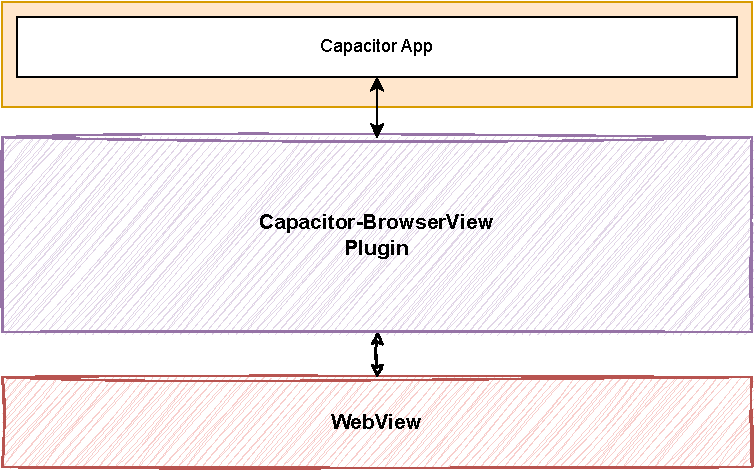
\includegraphics[width=0.8\textwidth]{assets/03_Capacitor-BrowserView/01_Zielsetzung.drawio.pdf}
  \caption[Capacitor-BrowserView / Zielsetzung]{Zielsetzung des Capacitor-BrowserView Plugins}
\end{figure}

Die vom Plugin implementierten Webbrowser"=Fenster bzw.\ unter Android und iOS genannten WebViews werden im Plugin als BrowserViews bezeichnet, um die Ähnlichkeit mit den bereits in Electron existierenden BrowserViews zu verdeutlichen.
\cite{android:api, ios:api, electron:docs}

\begin{note}
  Die offizielle Entwicklungsumgebung für iOS, Xcode, ist ausschließlich für macOS verfügbar.~\cite{xcode:support}
  Da während der Entwicklung nur Windows- und Linux-Geräte zur Verfügung standen, war das Implementieren und Testen des Plugins für iOS nicht möglich.
\end{note}

\subsection{Frontend und Backend}


\clearpage

\subsection{Gewählte Technologien}

\begin{figure}[H]
    \centering
    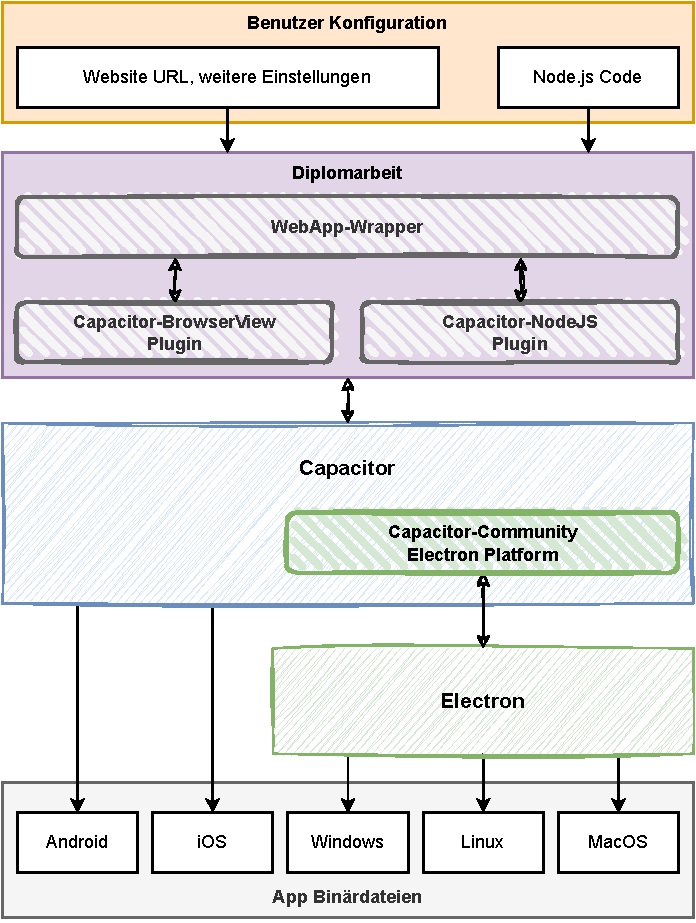
\includegraphics[width=\textwidth]{assets/01_Einführung/02_Zielsetzung+Frameworks.drawio.pdf}
\end{figure}


\clearpage

\subsection{Projekt-Aufbau}

\begin{figure}[H]
    \centering
    \includegraphics[width=\textwidth]{assets/01_Einführung/03_Aufbau.drawio.pdf}
\end{figure}

% https://capacitorjs.jp/blog/how-capacitor-works

\clearpage


\bigsection{Capacitor-NodeJS}
\addurlfn{event-emitter}{Event-Emitter}{https://nodejs.org/api/events.html}
\addurlfn{capacitor-electron-plattform}{Capacitor-Community Electron Plattform}{https://github.com/capacitor-community/electron}

\subsection{Zielsetzung}

Das Hauptziel des Capacitor-NodeJS Plugins ist die Entwicklung eines Plugins für Capacitor, welches es Entwicklern ermöglicht, Node.js Projekte in Capacitor Anwendungen zu integrieren.
Das Plugin soll eine \ac{api} bereitstellen, um zwischen der Node.js Runtime und der Anwendung zu kommunizieren.
Die \ac{api} soll an dem Node.js \fn{event-emitter} angelehnt werden, um die Kompatibilität mit vorhandenen Projekten zu verbessern.

\vspace{1em}

\begin{figure}[h]
    \centering
    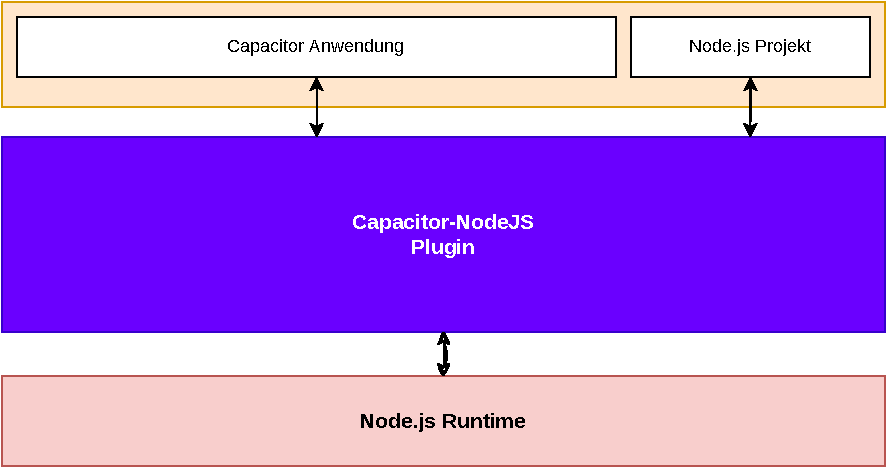
\includegraphics[width=\textwidth]{assets/02_Capacitor-NodeJS/01_Zielsetzung.drawio.pdf}
    \caption[Capacitor-NodeJS / Zielsetzung]{Zielsetzung des Capacitor-NodeJS Plugins}
\end{figure}

Als weiteres Ziel soll die Kompatibilität des Plugins mit der \fn{capacitor-electron-plattform} gewährleistet werden.
So soll das Plugin \textit{(und damit auch ein entsprechendes Node.js Projekt)} ohne zusätzlichen Aufwand sowohl in Mobile"=Anwendungen als auch in Desktop"=Anwendungen eingesetzt werden können.

\printfn

\subsection{Verwendete Bibliotheken}

Die Node.js Runtime wird zum Zeitpunkt dieser Arbeit offiziell nur auf gängigen Desktop"=Plattformen (Linux, Windows und macOS) unterstützt.~\cite{nodejs}
Daher musste für die Implementierung des Plugins zusätzlich zu den Plattform-\acsp{api} auf weitere Bibliotheken und Toolsets zurückgegriffen werden.

In diesem Abschnitt werden die Bibliotheken und Toolsets vorgestellt, die bei der Entwicklung des Capacitor-NodeJS Plugins verwendet wurden.

\subsubsection{Node.js for Mobile Apps}

Node.js for Mobile Apps ist ein Toolset für die Integration der Node.js Runtime in Mobile"=Anwendungen.
Das Hauptziel des Projekts ist es, Korrekturen sowie eine Bibliothek bereitzustellen, damit Node.js auch auf Mobile"=Plattformen (Android und iOS) problemlos ausgeführt werden kann.
\cite{nodejs-mobile, nodejs-mobile:docs}

Im Capacitor-NodeJS Plugin werden vom Projekt bereitgestellte Header-Dateien der mobilen Node.js Runtime sowie vorgefertigte native Binärdateien für Android und iOS verwendet.

\subsubsection{Android NDK}

Android \ac{ndk} ist ein Toolset, mit dem Teile einer Android Anwendung in nativem Code mit Sprachen wie C und C++ implementiert werden können.
Es bietet eine Reihe von Bibliotheken und Tools, die zur Erstellung von nativem Code für Android verwendet werden können.
\cite{android:ndk}

Damit Android Anwendungen nativen C oder C++ Code aufrufen können und umgekehrt, verwendet das Android \ac{ndk} das \ac{jni} Framework.
Dies bedeutet, dass Java-Code geschrieben werden kann, der auf Low"=Level"=Hardwarefunktionen zugreifen oder Funktionen in einer nativen Bibliothek aufrufen kann.
\cite{android:ndk}

Im Capacitor-NodeJS Plugin wird das Android \ac{ndk} benötigt, um auf die native JavaScript Runtime des Node.js for Mobile Apps Toolsets zuzugreifen.
\cite{nodejs-mobile:docs}

\subsection{Implementation}

\begin{figure}[H]
    \centering
    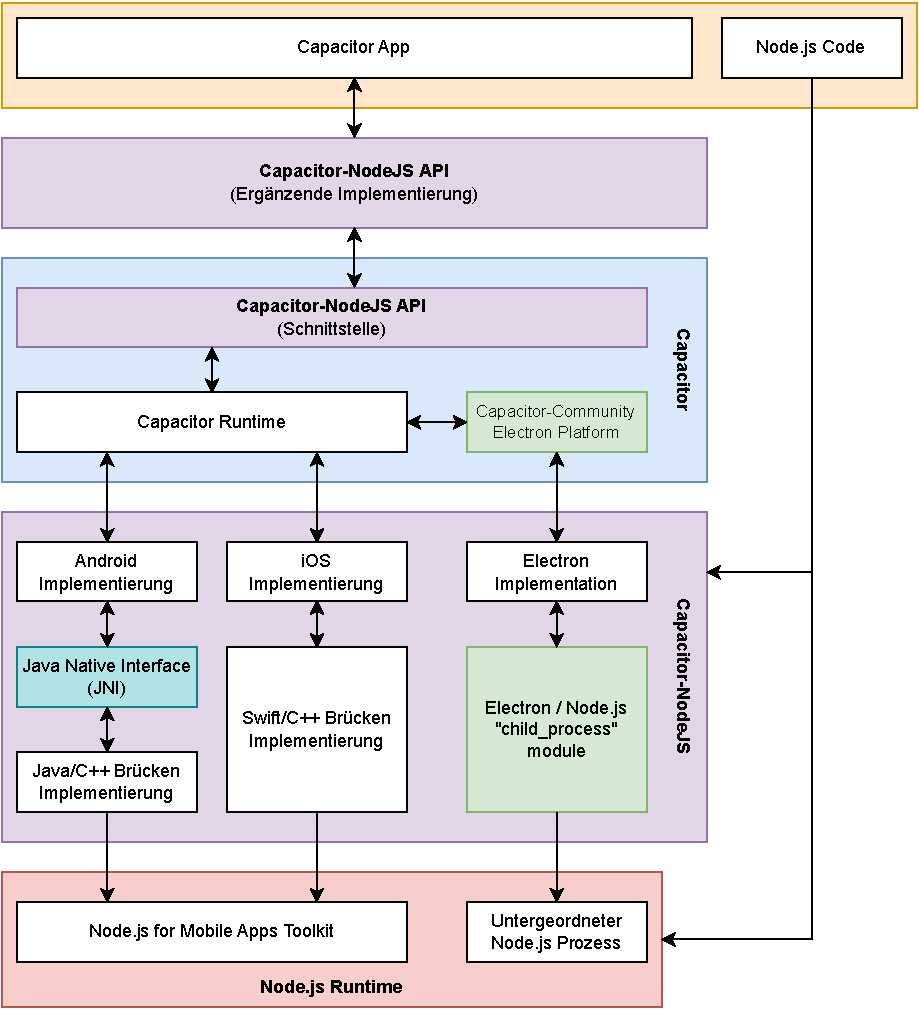
\includegraphics[width=\textwidth]{assets/02_Capacitor-NodeJS/03_Aufbau.drawio.pdf}
\end{figure}

% https://code.janeasystems.com/nodejs-mobile

\clearpage

\subsection{Benutzung}

In diesem Kapitel wird erklärt, wie das Plugin verwendet wird.

Um das Plugin für eine globale Zielgruppe zugänglich zu machen, wurde die Nachfolgende Dokumentation in englischer Sprache verfasst.

\vfill

\textbf{Table of contents}

\begin{itemize}
    \setlength\itemsep{-1em}
    \item \nameref{sec:Capacitor-NodeJS:Install}
    \item \nameref{sec:Capacitor-NodeJS:GettingStarted}
    \vspace{\itemsep}
    \begin{itemize}
        \setlength\itemsep{-1em}
        \item \nameref{sec:Capacitor-NodeJS:Basics}
        \item \nameref{sec:Capacitor-NodeJS:MinimalExample}
        \item \nameref{sec:Capacitor-NodeJS:InterprocessCommunication}
    \end{itemize}
    \item \nameref{sec:Capacitor-NodeJS:ComplexProjects}
    \vspace{\itemsep}
    \begin{itemize}
        \setlength\itemsep{-1em}
        \item \nameref{sec:Capacitor-NodeJS:CustomStartingPoint}
        \item \nameref{sec:Capacitor-NodeJS:InstallModules}
        \item \nameref{sec:Capacitor-NodeJS:ImproveLoadingTimes}
        \item \nameref{sec:Capacitor-NodeJS:ManualRuntimeStart}
    \end{itemize}
    \item \nameref{sec:Capacitor-NodeJS:MobileAPIDifferences}
    \item \nameref{sec:Capacitor-NodeJS:Configuration}
    \item \nameref{sec:Capacitor-NodeJS:API_BridgeModule}
    \item \nameref{sec:Capacitor-NodeJS:API_CapacitorLayer}
\end{itemize}

\vfill
\clearpage

\subsubsection{Install}
\label{sec:Capacitor-NodeJS:Install}

Capacitor v5 or newer is required. This project isn't compatible with lower versions of Capacitor.

\begin{minted}[breaklines,breakafter=/]{bash}
npm install https://github.com/hampoelz/capacitor-nodejs/releases/download/v1.0.0-beta.4/capacitor-nodejs.tgz
npx cap sync
\end{minted}

\begin{note}[Note]
  For now Android 32-bit x86 support is disabled since Capacitor-NodeJS \code{v1.0.0-beta.2} as there is currently no support for it in the latest version of the Node.js for Mobile Apps toolkit.
  \cite{nodejs-mobile}
\end{note}

\subsubsection{Getting Started}
\label{sec:Capacitor-NodeJS:GettingStarted}

This guide shows how to add a minimal Node.js project to a Capacitor application and communicate between these processes.

\paragraph{Basics}
\label{sec:Capacitor-NodeJS:Basics}

In the example below the Vite build system is used.
However, any build system can be used as long as the following criteria are met:

\begin{enumerate}
  \item The Node.js project (to be executed by the engine) must be located in a subdirectory named \code{nodejs} \textit{(or the path set via \code{nodeDir})} of the Capacitor \code{webDir}.
  \item The Node.js project must have a starting point, this can either be a script named \code{index.js} or a package.json with a \code{main} field.
\end{enumerate}

\begin{quote}
  For example if the Node.js project needs to be compiled or bundled then this output should be located in the subdirectory of the Capacitor \code{webDir}.
\end{quote}

\newpage

\paragraph{Minimal example}
\label{sec:Capacitor-NodeJS:MinimalExample}

In this example the directory for the app's source files is named \code{src}, the directory for static assets is named \code{static},
the directory for the compiled files is named \code{dist}, and the directory for the Node.js project is named \code{nodejs}.

So the configurations should contain at least the following values.~\cite{vite, capacitor:docs}

\textbf{Vite Configurations:}

\begin{minted}{typescript}
// in vite.config.js or vite.config.ts
{
  root: './src',
  publicDir: '../static',
  build: {
    outDir: '../dist'
  }
}
\end{minted}

\textbf{Capacitor Configurations:}

\begin{minted}{typescript}
// in capacitor.config.json or capacitor.config.ts
{
  "webDir": 'dist',
  "plugins": {
    "CapacitorNodeJS": {
      "nodeDir": "nodejs"
    }
  }
}
\end{minted}

\vspace{1em}

To meet the criteria from above using Vite, just create a new directory called \code{nodejs} inside the \code{static} directory.
And create a new file called \code{index.js} in it as the starting point.

\begin{quote}
  Vite will copy assets from the \code{static} directory to the root of the \code{dist} directory as-is.~\cite{vite}
  So the created \code{nodejs} project directory will be placed in the Capacitor \code{webdir} after build.
\end{quote}

\vspace{1em}

The project structure should now look something like this:

\begin{minted}{diff}
  capacitor-app/
  ├── ...
  ├── dist/                   # Capacitor webdir
  ├── src/                    # app source directory
+ ├── static/                 # static assets
+ │   ├── nodejs/             # Node.js project directory
+ │   │   ├── index.js        # Node.js main script
  ├── capacitor.config.json
  ├── vite.config.ts
  ├── ...
\end{minted}

\vspace{1em}

After building and syncing the project, the main script will be executed by the Node.js runtime when the application is launched.

A guide for a more complex Node.js project can be found in the \nameref{sec:Capacitor-NodeJS:ComplexProjects} section.

\paragraph{Interprocess Communication}
\label{sec:Capacitor-NodeJS:InterprocessCommunication}

A bridge module to communicate between the Capacitor layer and the Node.js process is built-in.

Use the following code in a Node.js script to wait for messages from the Capacitor layer and send messages back:

\begin{minted}{javascript}
const { channel } = require('bridge');

// Listens to "msg-from-capacitor" from the Capacitor layer.
channel.addListener('msg-from-capacitor', message => {
  console.log('[Node.js] Message from Capacitor: ' + message);
  
  // Sends a message back to the Capacitor layer.
  channel.send("msg-from-nodejs",
    `Replying to the message '${message}'.`,
    "And optionally add more arguments."
  );
});
\end{minted}

\vspace{1em}

Now it is possible to communicate with the Node.js process in the Capacitor application:

\begin{minted}{typescript}
import { NodeJS } from 'capacitor-nodejs';

// Listens to "msg-from-nodejs" from the Node.js process.
NodeJS.addListener('msg-from-nodejs', event => {
  document.body.innerHTML = `
    <p>
      <b>Message from Capacitor</b><br>
      First argument: ${event.args[0]}<br>
      Second argument: ${event.args[1]}
    </p>
  `;
  console.log(event);
});

// Waits for the Node.js process to initialize.
NodeJS.whenReady().then(() => {

  // Sends a message to the Node.js process.
  NodeJS.send({
    eventName: "msg-from-capacitor",
    args: [ "Hello from Capacitor!" ]
  });

});
\end{minted}

A full \ac{api} documentation can be found in the \nameref{sec:Capacitor-NodeJS:API_BridgeModule} section.

\clearpage

\subsubsection{Complex Projects}
\label{sec:Capacitor-NodeJS:ComplexProjects}

The examples in this guide are a continuation of the examples in the \nameref{sec:Capacitor-NodeJS:GettingStarted} guide.

\paragraph{Custom starting point}
\label{sec:Capacitor-NodeJS:CustomStartingPoint}

In the \nameref{sec:Capacitor-NodeJS:GettingStarted} guide, the default starting point \code{index.js} was used for the Node.js project.
However, the main script can be renamed or moved to subdirectories for a better organized project.

To change this starting point, add a file called \code{package.json} to the Node.js project, which describes the project more in detail.
Using the \code{main} field in this file, a custom starting point for the Node.js project can be specified.
This should be a module relative to the root of the Node.js project directory.
\cite{npm}

The package.json file could look like the following, if the \code{main} field is set to \code{server.js}:

\begin{minted}{javascript}
// static/nodejs/package.json
{
  "name": "capacitor-nodejs-project",
  "version": "1.0.0",
  "main": "./server.js"
}
\end{minted}

The project structure should then change to something like this:

\begin{minted}{diff}
  capacitor-app/
  ├── ...
  ├── dist/
  ├── src/
  ├── static/
  │   ├── nodejs/             # Node.js project directory
- │   │   ├── index.js        # main script (old)
+ │   │   ├── server.js       # main script (new)
+ │   │   ├── package.json    # starting point
  ├── capacitor.config.json
  ├── vite.config.ts
  ├── ...
\end{minted}

\newpage

\paragraph{Install Node.js Modules}
\label{sec:Capacitor-NodeJS:InstallModules}

To install Node.js modules, the project requires a \code{package.json} file.~\cite{npm}
See section \nameref{sec:Capacitor-NodeJS:CustomStartingPoint} for more details.

The modules have to be installed in the Node.js project directory in which the \code{package.json} file was created using the npm CLI\@.
After installing modules, rebuild and sync the Capacitor project to update the application with the Node.js project.

For convenience, a postinstall script can be added to the main \code{package.json} in the root of the Capacitor project to automatically install the modules of the Node.js project \cite{npm}:

\begin{minted}{javascript}
// package.json
{
  "scripts": {
    "postinstall": "cd static/nodejs/ && npm install"
  },
  // other config options
}
\end{minted}

\begin{quote}
  You may also want to add a gitignore file to ignore unnecessary files.
  To do this, create a new file called \code{.gitignore} in the Node.js project directory and copy the contents of \urlfn{\code{@github/gitignore}/Node.gitignore}{https://github.com/github/gitignore/blob/main/Node.gitignore} into it.
\end{quote}

\begin{important}[Important]
  If the \code{@capacitor-community/electron} plugin is used, packaging with the electron-builder may cause problems since it does not include the modules installed in the Node.js project by default. \cite{electron-builder}
  \\[1em]
  To fix this issue, add the configuration \code[javascript]{"includeSubNodeModules": true} to the \code{electron-builder.config.json}.
  \cite{electron-builder}
\end{important}

\newpage

\paragraph{Improve Node.js loading times}
\label{sec:Capacitor-NodeJS:ImproveLoadingTimes}

The Node.js project can quickly grow very large when installing modules.
For projects that contain a large number of files, the load time can be reduced by decreasing the number of files and the file sizes.
\cite{nodejs-mobile:docs}

For this reason, it is recommended to use bundler tools such as Rollup.js.
In the following example, Rollup is used to bundle the Node.js project with all its modules to a single file.
\cite{rollup, rollup-plugins}

To get started install Rollup and its plugins \enquote{commonjs}, \enquote{node-resolve} and \enquote{json} into the root of the Capacitor project.
If Vite is used as build system, Rollup is already pre-installed and does not need to be installed:

\begin{minted}{bash}
# Install Rollup (If Vite is used, this command is not needed)
npm i --save-dev rollup

# Install Rollup Plugins
npm i --save-dev @rollup/plugin-commonjs
npm i --save-dev @rollup/plugin-json
npm i --save-dev @rollup/plugin-node-resolve
\end{minted}

Since the Node.js project is now to be bundled, the project structure needs some changes.
The Node.js project should no longer be copied directly from Vite to the Capacitor webDir directory, instead it will be bundled with Rollup.

This means that the Node.js project directory needs to be moved from the static assets to somewhere else.
For example to the root directory of the Capacitor project:

\begin{minted}{diff}
  capacitor-app/
  ├── ...
  ├── dist/
  ├── src/
  ├── static/
- │   ├── nodejs/
- │   │   ├── node_modules/
- │   │   ├── server.js
- │   │   ├── package.json
- │   │   ├── ...
+ ├── nodejs/
+ │   ├── node_modules/
+ │   ├── server.js
+ │   ├── package.json
+ │   ├── ...
  ├── capacitor.config.json
  ├── vite.config.ts
  ├── ... 
\end{minted}

\begin{quote}
  Don't forget to update the new path to the project in the postinstall script,
  if one is used, as described in the \nameref{sec:Capacitor-NodeJS:InstallModules} section.
\end{quote}

\newpage

After the restructuring of the project, Rollup can be configured.
Create a new file called \code{rollup.config.mjs} with the following content \cite{rollup, rollup-plugins}:

\begin{minted}{typescript}
// rollup.config.mjs
import commonjs from '@rollup/plugin-commonjs';
import json from '@rollup/plugin-json';
import nodeResolve from '@rollup/plugin-node-resolve';

export default {
  input: 'nodejs/server.js',
  output: {
    file: 'dist/nodejs/index.js',
    format: 'cjs',
  },
  external: ['bridge'],
  plugins: [
    commonjs(),
    json(),
    nodeResolve({
      preferBuiltins: true,
    }),
  ],
}; 
\end{minted}

To add bundling of the Node.js project to the build steps, modify the main \code{package.json} in the root of the Capacitor project 
and add \code[bash]{&& rollup -c rollup.config.mjs} to the \code{build} entry in the \code{scripts} object \cite{npm, rollup}:

\begin{minted}{diff}
# package.json
{
  "scripts": {
-   "build": "vite build"
+   "build": "vite build && rollup -c rollup.config.mjs"
  }
}
\end{minted}

So the project structure should look something like this:

\begin{minted}{diff}
  capacitor-app/
  ├── ...
  ├── dist/
  ├── src/
  ├── nodejs/
  │   ├── node_modules/
  │   ├── server.js
  │   ├── package.json
  │   ├── ...
  ├── capacitor.config.json
+ ├── rollup.config.mjs
  ├── vite.config.ts
  ├── ... 
\end{minted}

After building and syncing the project, the Node.js runtime should start faster now.

\newpage

\paragraph{Manual Node.js runtime start}
\label{sec:Capacitor-NodeJS:ManualRuntimeStart}

By default, the Node.js runtime starts automatically with application start.
However, this behavior may not be suitable for all projects.

This behavior can be disabled globally via the \code{startMode} plugin configuration:

\begin{minted}{diff}
# in capacitor.config.json or capacitor.config.ts
{
  "webDir": 'dist',
  "plugins": {
    "CapacitorNodeJS": {
      "nodeDir": "nodejs",
+     "startMode": "manual",
    },
  },
} 
\end{minted}

Now the Node.js runtime has to be started manually with the \code{NodeJS.start()} command:

\begin{minted}{typescript}
import { NodeJS } from 'capacitor-nodejs';

// Starts the Node.js engine
NodeJS.start();

// Waits for the Node.js process to initialize
NodeJS.whenReady().then(() => {
  // Communicate with the Node.js process
});
\end{minted}

Manually starting the Node.js runtime provides options to override the \code{nodeDir} configuration or even the path for the main script.

In addition, arguments can be passed to the main script and environment variables for the Node.js runtime can be set:

\begin{minted}{typescript}
import { NodeJS } from 'capacitor-nodejs';

// Options for starting the Node.js engine manually
const options = {
  args: [ "--option", "value" ],
  env: {
    "DB_HOST": "localhost",
    "DB_USER": "myuser",
    "DB_PASS": "mypassword"
  }
}

// Starts the Node.js engine with properties as set by the `options`
NodeJS.start(options);
\end{minted}

\begin{note}[Note]
  Due to limitations in the Node.js for Mobile Apps toolkit, restarting the runtime after it has finished is not supported.
  \cite{nodejs-mobile:docs}
\end{note}

\newpage

\paragraph{Data storage}
\label{sec:Capacitor-NodeJS:DataStorage}

Mobile platforms are different than the usual desktop platforms in that they require applications to write in specific sandboxed paths and don't have permissions to write elsewhere.
\cite{nodejs-mobile:docs}

The built-in bridge module provides an \ac{api} to get a per-user application data directory on each platform:

\begin{minted}{javascript}
const { getDataPath } = require('bridge');

// Get a path where data can be read and written
const dataPath = getDataPath();
\end{minted}

\begin{warning}[Warning]
  Do not use the Node.js project directory itself for data storage, it will be overwritten after each application update!
  \cite{nodejs-mobile:docs}
\end{warning}

To get a path for temporary files, the node.js inbuilt method \code{os.tmpdir()} can be used \cite{nodejs}:

\begin{minted}{javascript}
const os = require('os');

// Get a path for temporary files
const tmpPath = os.tmpdir();
\end{minted}

\begin{warning}[Warning]
  On Android, the files in the cache are kept until the system needs space, so it increases the application's disk space unless the developer manually deletes them.
  \cite{nodejs-mobile:docs}
\end{warning}

\clearpage

\subsubsection{Mobile Node.js APIs differences}
\label{sec:Capacitor-NodeJS:MobileAPIDifferences}

\begin{note}[Note]
  This section is based on the documentation of the Node.js for Mobile Apps toolkits.
  \cite{nodejs-mobile:docs}
\end{note}

Not every \ac{api} is supported on mobile devices.
Mobile operating systems do not allow applications to call certain \acsp{api} that are expected to be available on other operating systems.

\paragraph{child\_process module}

Mobile applications are expected to be a single process.
\acsp{api} that create new processes, such as \code{child_process.spawn()} or \code{child_process.fork()} will therefore run into permission issues.

\paragraph{file system (fs) module}

On mobile platforms, the current working directory is the root directory of the file system.
This can lead to unexpected behavior in code that assumes that the current working directory is set to the directory of the Node.js project.

On Android creating hard links (\code{fs.link()} and \code{fs.linkSync()}) is not supported.

\paragraph{internationalization (intl) module}

The internationalization (\code{intl}) module is not available on current nodejs-mobile builds.

\paragraph{os module}

\begin{itemize}
  \setlength\itemsep{-0.5em}
  \item \code{os.cpus()} may return inconsistent/unreliable results, since different OS versions will have different permissions for accessing CPU information.
  \item \code{os.homedir()} on mobile platforms there is no concept of user home directories.
  \item \code{os.platform()} can also return \enquote{android} or \enquote{ios}, depending on the platform.
\end{itemize}

On Android, the files in the cache (\code{os.tmpdir()}) are kept until the system needs space, so it increases the application's disk space unless the developer manually deletes them.

\newpage

\paragraph{process module}

\begin{itemize}
  \setlength\itemsep{-0.5em}
  \item \code{process.cwd()} is the root directory of the file system, instead of the start directory of the project.
  \item \code{process.exit()} is not allowed by the Apple AppStore guildelines.
  \item \code{process.stdin} is not available.
  \item \code{process.platform} can also be \enquote{android} or \enquote{ios}, depending on the platform.
  \item \code{process.versions} includes the \enquote{mobile} key, containing the nodejs-mobile core library version.
\end{itemize}

The following functions are only available on POSIX platforms, so they are unavailable on Android:

\begin{itemize}
  \setlength\itemsep{-0.8em}
  \item \code{process.getegid()}
  \item \code{process.geteuid()}
  \item \code{process.getgid()}
  \item \code{process.getgroups()}
  \item \code{process.getuid()}
  \item \code{process.setegid()}
  \item \code{process.seteuid()}
  \item \code{process.setgid()}
  \item \code{process.setgroups()}
  \item \code{process.setuid()}
\end{itemize}

\clearpage

\subsubsection{Configuration}
\label{sec:Capacitor-NodeJS:Configuration}

These config values are available:

\begin{config}{Capacitor-NodeJS / Configuration}
  \code{nodeDir}   & \code[typescript]{string} & Relative path of the integrated Node.js project based on the Capacitor webdir. Defaults to \code[typescript]{"nodejs"}. \\ \hline
  \code{startMode} & \code[typescript]{string} & Startup mode of the Node.js engine. Defaults to \code[typescript]{"auto"}. The following values are accepted: \\
                   &                           & \textbf{\code{auto}}: The Node.js engine starts automatically when the application is launched. \\
                   &                           & \textbf{\code{manual}}: The Node.js engine is started via the \code{NodeJS.start()} method. \\ \hline
\end{config}
  
\textbf{Examples}

In \code{capacitor.config.json}:

\begin{minted}{json}
{
  "plugins": {
    "CapacitorNodeJS": {
      "nodeDir": "custom-nodejs",
      "startMode": "manual"
    }
  }
}
\end{minted}

In \code{capacitor.config.ts}:

\begin{minted}{typescript}
/// <reference types="capacitor-nodejs" />

import { CapacitorConfig } from '@capacitor/cli';

const config: CapacitorConfig = {
  plugins: {
    CapacitorNodeJS: {
      nodeDir: "custom-nodejs",
      startMode: "manual",
    },
  },
};

export default config;
\end{minted}

\clearpage

\subsubsection{API - Bridge module}
\label{sec:Capacitor-NodeJS:API_BridgeModule}

The \code{bridge} module is built-in.
It provides an \ac{api} to communicate between the Capacitor layer and the Node.js process, as well as an \ac{api} to get a per-user application data directory on each platform.

TypeScript declarations for this \code{bridge} module can be manually installed as dev-dependency.
If needed, the types-only package can be found under \code{node_modules/capacitor-nodejs/assets/types/bridge} in the root of the Capacitor project.

% -------------------- %

\begin{itemize}
  \setlength\itemsep{-0.8em}
  \item \code{getDataPath()}
  \item \code{channel}
\end{itemize}

% -------------------- %

\paragraph{getDataPath()}

\begin{minted}{typescript}
  getDataPath: () => string
\end{minted}

Returns a path for a per-user application data directory on each platform, where data can be read and written.

% -------------------- %

\paragraph{channel}

The \code{channel} class of the \code{bridge} module is an Event-Emitter.
It provides a few methods to send messages from the Node.js process to the Capacitor layer, and to receive replies from the Capacitor layer.

It has the following method to listen for events and send messages:

\begin{itemize}
  \setlength\itemsep{-0.8em}
  \item \code{send(...)}
  \item \code{on(string, ...)}
  \item \code{once(string, ...)}
  \item \code{addListener(string, ...)}
  \item \code{removeListener(...)}
  \item \code{removeAllListeners(...)}
\end{itemize}

% -------------------- %

\paragraph{channel.send(...)}

\begin{minted}{typescript}
  send: (
    eventName: string,
    ...args: any[]
  ) => void
\end{minted}

Sends a message to the Capacitor layer via \code{eventName}, along with arguments.
Arguments will be serialized with \ac{json}.

\begin{itemize}
  \setlength\itemsep{-0.8em}
  \item \code{eventName}: The name of the event being send to.
  \item \code{args}: The Array of arguments to send.
\end{itemize}

% -------------------- %

\paragraph{channel.on(string, ...)}

\begin{minted}{typescript}
  on: (
    eventName: string,
    listener: (...args: any[]) => void
  ) => void
\end{minted}

Listens to \code{eventName} and calls \code{listener(args...)} when a new message arrives from the Capacitor layer.

\begin{itemize}
  \setlength\itemsep{-0.8em}
  \item \code{args}: The received array of arguments.
\end{itemize}

% -------------------- %

\paragraph{channel.once(string, ...)}

\begin{minted}{typescript}
  once: (
    eventName: string,
    listener: (...args: any[]) => void
  ) => void
\end{minted}

Listens one time to \code{eventName} and calls \code{listener(args...)} when a new message arrives from the Capacitor layer, after which it is removed.

\begin{itemize}
  \setlength\itemsep{-0.8em}
  \item \code{args}: The received array of arguments.
\end{itemize}

% -------------------- %

\paragraph{channel.addListener(string, ...)}

\begin{minted}{typescript}
  addListener: (
    eventName: string,
    listener: (...args: any[]) => void
  ) => void
\end{minted}

Alias for \code{channel.on(string, ...)}.

% -------------------- %

\paragraph{channel.removeListener(...)}

\begin{minted}{typescript}
  removeListener: (
    eventName: string,
    listener: (...args: any[]) => void
  ) => void
\end{minted}

Removes the specified \code{listener} from the listener array for the specified \code{eventName}.

% -------------------- %

\paragraph{channel.removeAllListeners(...)}

\begin{minted}{typescript}
  removeAllListeners: (
    eventName?: string
  ) => void
\end{minted}

Removes all listeners, or those of the specified \code{eventName}.

\begin{itemize}
  \setlength\itemsep{-0.8em}
  \item \code{eventName}: The name of the event all listeners will be removed from.
\end{itemize}

% -------------------- %

\clearpage

\subsubsection{API - Capacitor layer}
\label{sec:Capacitor-NodeJS:API_CapacitorLayer}

The \code{NodeJS} module is the \ac{api} used in the Capacitor app.
It provides a few methods to send messages from the Node.js layer and wait for them.

It has the following methods:

\begin{itemize}
  \setlength\itemsep{-0.8em}
  \item \code{start(...)}
  \item \code{send(...)}
  \item \code{whenReady()}
  \item \code{addListener(string, ...)}
  \item \code{removeListener(...)}
  \item \code{removeAllListeners(...)}
  \item Interfaces
  \item Type Aliases
\end{itemize}

% -------------------- %

\paragraph{start(...)}

\begin{minted}{typescript}
  start(
    options?: StartOptions
  ) => Promise<void>
\end{minted}

Starts the Node.js engine with properties as set by the \code{options}.

\textbf{Note:} This method is only available if the Node.js engine startup mode was set to \code[typescript]{'manual'} via the plugin configuration.

% -------------------- %

\paragraph{send(...)}

\begin{minted}{typescript}
  send(
    args: ChannelPayloadData
  ) => Promise<void>
\end{minted}

Sends a message to the Node.js process.

% -------------------- %

\paragraph{whenReady()}

\begin{minted}{typescript}
  whenReady() => Promise<void>
\end{minted}

Resolves when the Node.js process is initialized.

% -------------------- %

\newpage

\paragraph{addListener(string, ...)}

\begin{minted}{typescript}
  addListener(
    eventName: string,
    listenerFunc: ChannelListenerCallback
  ) => Promise<PluginListenerHandle> & PluginListenerHandle
\end{minted}

Listens to \code{eventName} and calls \code{listenerFunc(data)} when a new message arrives from the Node.js process.

\textbf{Note:} When using the Electron platform, \code{PluginListenerHandle.remove()} does not work due to limitations.~\cite{capacitor-electron}
Use \code{removeListener(listenerFunc)} instead.

\textbf{Returns:} \code[typescript]{Promise<PluginListenerHandle> & PluginListenerHandle}

% -------------------- %

\paragraph{removeListener(...)}

\begin{minted}{typescript}
  removeListener(
    listenerHandle: PluginListenerHandle
  ) => Promise<void>
\end{minted}

Removes the specified \code{listenerHandle} from the listener array for the event it refers to.

% -------------------- %

\paragraph{removeAllListeners(...)}

\begin{minted}{typescript}
  removeAllListeners(
    eventName?: string
  ) => Promise<void>
\end{minted}

Removes all listeners, or those of the specified \code{eventName}, for this plugin.

% -------------------- %

\newpage

\paragraph{Interfaces}


\subparagraph{StartOptions}

An interface containing the options used when starting the Node.js engine manually.

\begin{interfacedesc}{Capacitor-NodeJS / StartOptions}[5em]
  \code{nodeDir} & \code[typescript]{string}   & Relative path of the integrated Node.js project based on the Capacitor webdir. Defaults to the \code{nodeDir} field of the global plugin configuration. If the \code{nodeDir} config is not set, \code{nodejs} in the Capacitor webdir is used as Node.js project directory. \\ \hline
  \code{script}  & \code[typescript]{string}   & The primary entry point to the Node.js program. This should be a module relative to the root of the Node.js project folder. Defaults to the \code{main} field in the project's package.json. If the \code{main} field is not set, \code{index.js} in the project's root folder is used. \\ \hline
  \code{args}    & \code[typescript]{string[]} & A list of string arguments. \\ \hline
  \code{env}     & \code[typescript]{NodeEnv}  & Environment key-value pairs. \\ \hline
\end{interfacedesc}

% -------------------- %

\subparagraph{NodeEnv}

An interface that holds environment variables as string key-value pairs.

% -------------------- %

\subparagraph{ChannelPayloadData}

The payload data to send a message to the web page via \code{eventName},
along with arguments. Arguments will be serialized with \ac{json}.

\begin{interfacedesc}{Capacitor-NodeJS / ChannelPayloadData}
  \code{eventName} & \code[typescript]{string} & The name of the event being send to. \\ \hline
  \code{args}      & \code[typescript]{any[]}  & The array of arguments to send. \\ \hline
\end{interfacedesc}   

% -------------------- %

\subparagraph{PluginListenerHandle}

\begin{interface}{Capacitor-NodeJS / PluginListenerHandle}
  \code{remove} & \code[typescript]{() => Promise<void>} \\ \hline
\end{interface}

% -------------------- %

\subparagraph{ChannelCallbackData}

The callback data object when a message from the Node.js process arrives.

\begin{interfacedesc}{Capacitor-NodeJS / ChannelCallbackData}
  \code{args} & \code[typescript]{any[]} & The received array of arguments. \\ \hline
\end{interfacedesc}

% -------------------- %

\paragraph{Type Aliases}


\subparagraph{ChannelListenerCallback}

The callback function to be called when listen to messages from the Node.js process.

\code[typescript]{(data: ChannelCallbackData): void}



\bigsection{Capacitor-BrowserView}
\subsection{Zielsetzung}

Das Hauptziel des Capacitor-BrowserView Plugins ist die Entwicklung eines Plugins für Capacitor, welches Entwicklern ermöglicht, zusätzliche Webbrowser"=Fenster (WebViews) innerhalb einer Capacitor"=Anwendung zu erstellen und zu steuern.
Diese Fenster können zum Anzeigen und Manipulieren von zusätzlichen Webinhalten verwendet werden.
Dies ist praktisch, um externe Inhalte dynamisch anzuzeigen und von der Capacitor"=Anwendung zu isolieren.

Darüber hinaus soll eine optional zu aktivierende Kommunikation zwischen geladenen Webinhalten und der Capacitor"=Anwendung ermöglicht werden.
Dies ist sinnvoll, wenn ein vertrauenswürdiger externer Inhalt geladen wird, der nicht vollständig isoliert werden soll, da ein Datenaustausch mit diesem Inhalt und der Capacitor"=Anwendung benötigt wird.

Das Plugin soll ohne zusätzlichen Aufwand sowohl in Mobile- als auch in Desktop"=Anwendungen eingesetzt werden können.

\begin{figure}[H]
  \centering
  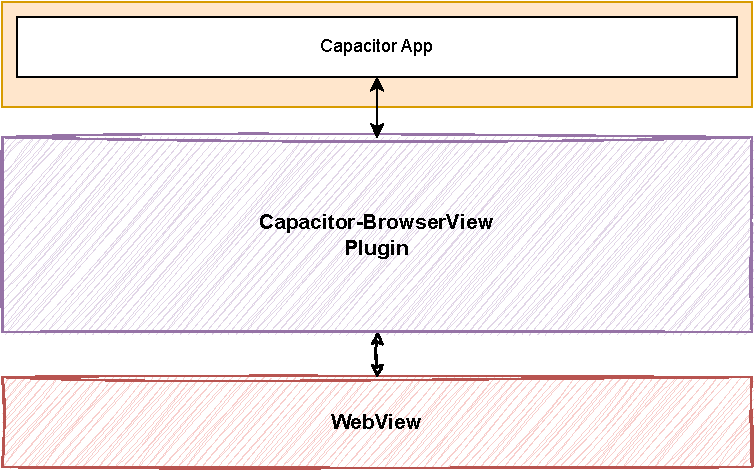
\includegraphics[width=0.8\textwidth]{assets/03_Capacitor-BrowserView/01_Zielsetzung.drawio.pdf}
  \caption[Capacitor-BrowserView / Zielsetzung]{Zielsetzung des Capacitor-BrowserView Plugins}
\end{figure}

Die vom Plugin implementierten Webbrowser"=Fenster bzw.\ unter Android und iOS genannten WebViews werden im Plugin als BrowserViews bezeichnet, um die Ähnlichkeit mit den bereits in Electron existierenden BrowserViews zu verdeutlichen.
\cite{android:api, ios:api, electron:docs}

\begin{note}
  Die offizielle Entwicklungsumgebung für iOS, Xcode, ist ausschließlich für macOS verfügbar.~\cite{xcode:support}
  Da während der Entwicklung nur Windows- und Linux-Geräte zur Verfügung standen, war das Implementieren und Testen des Plugins für iOS nicht möglich.
\end{note}

\subsection{Implementation}

\begin{figure}[H]
    \centering
    \includegraphics[width=\textwidth]{assets/03_Capacitor-BrowserView/03_Aufbau.drawio.pdf}
\end{figure}


\clearpage

\subsection{Interprozesskommunikation}

\begin{figure}[H]
    \centering
    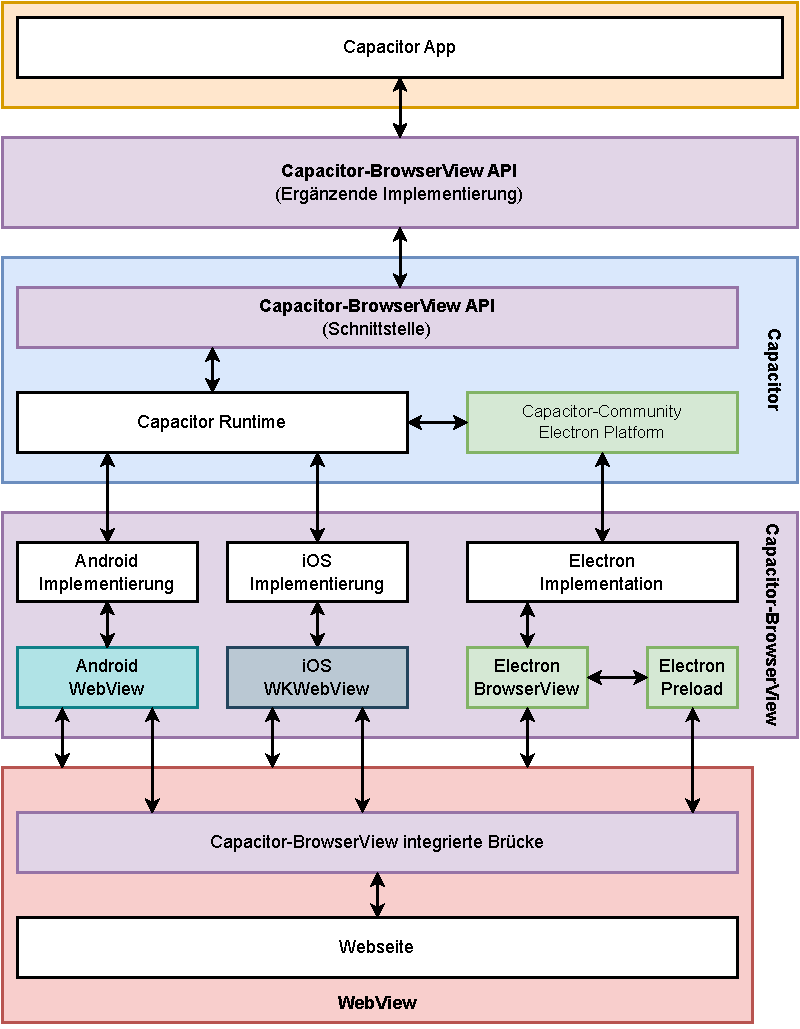
\includegraphics[width=\textwidth]{assets/03_Capacitor-BrowserView/04_Aufbau+IPC.drawio.pdf}
\end{figure}


\clearpage

\subsection{Benutzung}

In diesem Kapitel wird Schritt für Schritt erklärt, wie das Plugin verwendet wird.
Es enthält Beispiele für einfache und komplexe Projekte sowie entsprechende \acs{api}"=Dokumentationen.

Dieser Teil der Dokumentation bezieht sich auf die Vorabversion \code{1.0.0-beta.3} des Plugins.
Die neueste Version und die dazugehörige Dokumentation sind auf der \href{https://github.com/hampoelz/Capacitor-BrowserView}{GitHub-Projektseite}\footnotemark[0] zu finden.

Um das Plugin für eine globale Zielgruppe zugänglich zu machen, wurde die Nachfolgende Dokumentation in englischer Sprache verfasst.

\footnotetext[0]{\url{https://github.com/hampoelz/Capacitor-BrowserView}}

\vspace{3em}

\textbf{Table of contents}

\begin{itemize}
    \setlength\itemsep{-1em}
    \item \hyperref[sec:Capacitor-BrowserView:GettingStarted]{Getting Started}
    \vspace{\itemsep}
    \begin{itemize}
        \setlength\itemsep{-1em}
        \item \hyperref[sec:Capacitor-BrowserView:MinimalExample]{Minimal example}
        \item \hyperref[sec:Capacitor-BrowserView:InterprocessCommunication]{Inter-Process Communication}
    \end{itemize}
    \item \hyperref[sec:Capacitor-BrowserView:Configuration]{Configuration}
    \item \hyperref[sec:Capacitor-BrowserView:API_BridgeModule]{API - Bridge module}
    \item \hyperref[sec:Capacitor-BrowserView:API_CapacitorLayer]{API - Capacitor layer}
\end{itemize}

\newpage

\subsubsection{Getting Started}
\label{sec:Capacitor-BrowserView:GettingStarted}

This guide shows how to add a BrowserView to a Capacitor application and communicate with the web page.

\paragraph{Minimal example}
\label{sec:Capacitor-BrowserView:MinimalExample}

To embed an additional web page to the Capacitor app, first a new BrowserView needs to be created.
This is done by importing the BrowserView class from the Capacitor-BrowserView plugin and calling the create method.
After that, just set its bounds and load a website.

\begin{minted}{typescript}
import { BrowserView } from 'capacitor-browserview';

// Creates a new BrowserView, sets its bounds and loads a website.
const myView = await BrowserView.create();
myView.setBounds({ bounds: { x: 0, y: 0, width: 300, height: 600 } });
myView.loadUrl({ url: "https://capacitorjs.com/" });
\end{minted}

At this point, the BrowserView should be created within the application and the website should start loading.
Using the returned reference to the BrowserView, it is easy to interact with it, as shown here in a few examples:

\begin{minted}{typescript}
// Reloads the current web page.
myView.reload();

// Gets the user-agent for this web page.
const { userAgent } = await myView.getUserAgent();
console.log("The following UserAgent is used for this web page: "
    + userAgent);

// Handles finished page load.
myView.addListener('did-finish-load', () => {
    console.log("Congratulations! The web page loaded successfully.");
});

// Handles title changes of the web page.
myView.addListener('page-title-updated', event => {
    console.log(`The web page has changed its title to '${event.title}'.`);
});

// Removes the BrowserView from the app, and cleans up references.
myView.destroy();
\end{minted}

\newpage

\paragraph{Inter-Process Communication}
\label{sec:Capacitor-BrowserView:InterprocessCommunication}

This plugin includes a bridge between the Capacitor layer and the loaded web page in the BrowserView(s).
However, this feature is disabled by default. It can be enabled either globally via the plugin configuration or for each BrowserView individually during its creation.

If the bridge feature is enabled, the global object \code[javascript]{window.CapacitorBrowserView} is available on web pages within the corresponding BrowserView.

To use the bridge, the website first needs to be modified so that it is capable of receiving and returning messages.
For example, add the following sample code to the web page:

\begin{minted}{javascript}
// Listens to "msg-from-capacitor" from the Capacitor layer.
CapacitorBrowserView.addListener("msg-from-capacitor", message => {
    console.log('Message from Capacitor-App: ' + message);

    // Sends a message back to the Capacitor layer.
    CapacitorBrowserView.send("msg-from-web",
        `Replying to the message '${message}'.`,
        "And optionally add further args"
    );
});
\end{minted}

After that, a new BrowserView with an enabled bridge needs be set up.
In addition, the Capacitor app should also be able to receive messages and send a message to the website.
Note that the web page must be loaded entirely before it can receive messages.
This could look something like this:

\begin{minted}{typescript}
import { BrowserView } from 'capacitor-browserview';

const myView = await BrowserView.create({ enableBridge: true });
myView.setBounds({ bounds: { x: 0, y: 0, width: 300, height: 600 } });

// Listens to "msg-from-web" from the web page.
myView.addMessageListener('msg-from-web', data => {
    console.log("Message from web page: ", data.args);
});

// Waits for the web page to finish loading.
myView.addListener('did-finish-load', () => {

    // Sends a message to the web page.
    myView.sendMessage({
        eventName: "msg-from-capacitor",
        args: [ "Hello from Capacitor!" ]
    });

});

myView.loadUrl({ url: "https://webpage.dev/" });
\end{minted}

A full \ac{api} documentation can be found in the \hyperref[sec:Capacitor-BrowserView:API_BridgeModule]{API - Bridge module} section.

\clearpage

\addurlfn{mixed-content}{Mixed content}{https://developer.mozilla.org/en-US/docs/Web/Security/Mixed_content}

\subsubsection{Configuration}
\label{sec:Capacitor-BrowserView:Configuration}

The following configurations are applied globally to all BrowserViews.
However, most of them can be overridden individually when a BrowserView is created or changed later via methods.

These config values are available:

\begin{config}[Capacitor-BrowserView / Configuration]
  \code{url}                  & \code[typescript]{string}   & Default external \ac{url} loaded in BrowserViews. \\ \hline
  \code{allowMultipleWindows} & \code[typescript]{boolean}  & Open links that request a new tab or window in the external browser instead of the BrowserViews. \\
                              &                             & Defaults to \code[typescript]{true} \\ \hline
  \code{allowNavigation}      & \code[typescript]{string[]} & Set regular expressions to which the BrowserViews can navigate additional. By default, all external \acp{url} are opened in the external browser (not the BrowserView). \\
                              &                             & Defaults to \code[typescript]{[]} \\ \hline
  \code{enableBridge}         & \code[typescript]{boolean}  & Enable a bridge between the Capacitor layer and the loaded web page. \\
                              &                             & Defaults to \code[typescript]{false} \\ \hline
  \code{overrideUserAgent}    & \code[typescript]{string}   & Default user-agent for BrowserViews. \\ \hline
  \code{appendUserAgent}      & \code[typescript]{string}   & String to append to the original user-agent for BrowserViews. This is disregarded if \code{overrideUserAgent} is used. \\ \hline
  \code{backgroundColor}      & \code[typescript]{Color}    & Default background color for BrowserViews. \\ \hline
\end{config}

\begin{config}[Capacitor-BrowserView / Configuration (Android)]
  \codebreak{android}{OverrideUserAgent} & \code[typescript]{string}   & Overrides global \code{overrideUserAgent} option on Android. \\ \hline
  \codebreak{android}{AppendUserAgent}   & \code[typescript]{string}   & Overrides global \code{appendUserAgent} option on Android. \\ \hline
  \codebreak{android}{BackgroundColor}   & \code[typescript]{Color}    & Overrides global \code{backgroundColor} option on Android. \\ \hline
  \codebreak{android}{AllowMixedContent} & \code[typescript]{boolean}  & Enable mixed content in the BrowserViews for Android. \fn{mixed-content} is disabled by default for security. During development, this option may need to be enabled to allow the BrowserViews to load files from different schemes. \\
                                         &                             & \textbf{This is not intended for use in production.} \\ 
                                         &                             & Defaults to \code[typescript]{false} \\ \hline
\end{config}

\begin{config}[Capacitor-BrowserView / Configuration (Electron)]
  \codebreak{electron}{OverrideUserAgent} & \code[typescript]{string}   & Overrides global \code{overrideUserAgent} option on Electron. \\ \hline
  \codebreak{electron}{AppendUserAgent}   & \code[typescript]{string}   & Overrides global \code{appendUserAgent} option on Electron. \\ \hline
  \codebreak{electron}{BackgroundColor}   & \code[typescript]{Color}    & Overrides global \code{backgroundColor} option  on Electron. \\ \hline
  \codebreak{electron}{AllowMixedContent} & \code[typescript]{boolean}  & Enable mixed content in the BrowserViews for Electron. \fn{mixed-content} is disabled by default for security. During development, this option may need to be enabled to allow the BrowserViews to load files from different schemes. \\
                                          &                             & \textbf{This is not intended for use in production.} \\ 
                                          &                             & Defaults to \code[typescript]{false} \\ \hline
\end{config}

\newpage

\textbf{Examples}

In \code{capacitor.config.json}:

\begin{minted}{json}
{
  "plugins": {
    "CapacitorBrowserView": {
      "url": "https://capacitorjs.com/",
      "allowMultipleWindows": false,
      "allowNavigation": [
        "capacitorjs\.com",
        "ionic\.io\/blog\/.*capacitor.*"
      ],
      "enableBridge": true,
      "overrideUserAgent": "Mozilla/5.0 (CapacitorJS) CapacitorApp/1.0",
      "appendUserAgent": "CapacitorApp/1.0",
      "backgroundColor": "#ffffff",
      "androidOverrideUserAgent": "Mozilla/5.0 (Android) CapacitorApp/1.0",
      "androidAppendUserAgent": "CapacitorApp/1.0 (Android)",
      "androidBackgroundColor": "#ffffff",
      "androidAllowMixedContent": false,
      "electronOverrideUserAgent": "Mozilla/5.0 (Electron) CapacitorApp/1.0",
      "electronAppendUserAgent": "CapacitorApp/1.0 (Electron)",
      "electronBackgroundColor": "#ffffff",
      "electronAllowMixedContent": false
    }
  }
}
\end{minted}

In \code{capacitor.config.ts}:

\begin{minted}{typescript}
/// <reference types="capacitor-browserview" />

import { CapacitorConfig } from '@capacitor/cli';

const config: CapacitorConfig = {
  plugins: {
    CapacitorBrowserView: {
      url: "https://capacitorjs.com/",
      allowMultipleWindows: false,
      allowNavigation: [
        "capacitorjs\.com",
        "ionic\.io\/blog\/.*capacitor.*"
      ],
      enableBridge: true,
      overrideUserAgent: "Mozilla/5.0 (CapacitorJS) CapacitorApp/1.0",
      appendUserAgent: "CapacitorApp/1.0",
      backgroundColor: "#ffffff",
      androidOverrideUserAgent: "Mozilla/5.0 (Android) CapacitorApp/1.0",
      androidAppendUserAgent: "CapacitorApp/1.0 (Android)",
      androidBackgroundColor: "#ffffff",
      androidAllowMixedContent: false,
      electronOverrideUserAgent: "Mozilla/5.0 (Electron) CapacitorApp/1.0",
      electronAppendUserAgent: "CapacitorApp/1.0 (Electron)",
      electronBackgroundColor: "#ffffff",
      electronAllowMixedContent: false,
    },
  },
};

export default config;
\end{minted}

\printfn

\clearpage

\subsubsection{API - Bridge module}
\label{sec:Capacitor-BrowserView:API_BridgeModule}

This plugin includes a bridge between the Capacitor layer and the loaded web page in the BrowserView(s).
However, this feature is disabled by default. It can be enabled either globally via the plugin configuration or for each BrowserView individually during its creation.

If the bridge feature is enabled, the global object \code[javascript]{window.CapacitorBrowserView} is available on web pages within the corresponding BrowserView.

The \code[javascript]{window.CapacitorBrowserView} object provides an \ac{api} to communicate between the Capacitor layer and the web pages.

It has the following methods to listen for events and send messages:

\begin{itemize}
  \setlength\itemsep{-0.8em}
  \item \code{send(...)}
  \item \code{addListener(string, ...)}
\end{itemize}

% -------------------- %

\paragraph{CapacitorBrowserView.send(...)}

\begin{minted}{typescript}
  send: (
    eventName: string,
    ...args: any[]
  ) => void
\end{minted}

Sends a message to the Capacitor layer via \code{eventName}, along with arguments.
Arguments will be serialized with \ac{json}.

\begin{itemize}
  \setlength\itemsep{-0.8em}
  \item \code{eventName}: The name of the event being send to.
  \item \code{args}: The Array of arguments to send.
\end{itemize}

% -------------------- %

\paragraph{CapacitorBrowserView.addListener(string, ...)}

\begin{minted}{typescript}
  addListener: (
    eventName: string,
    callback: (...args: any[]) => void
  ) => void
\end{minted}

Listens to \code{eventName} and calls \code{callback(args...)} when a new message arrives from the Capacitor layer.

\begin{itemize}
  \setlength\itemsep{-0.8em}
  \item \code{args}: The received array of arguments.
\end{itemize}

% -------------------- %

\clearpage

\subsubsection{API - Capacitor layer}
\label{sec:Capacitor-BrowserView:API_CapacitorLayer}

\begin{note}[Note]
  The following documentation is based on parts of the Android WebView and Electron BrowserView documentation.
  \cite{android:api, electron}
\end{note}

A \code{BrowserView} can be used to embed additional web content into the Capacitor-App.
It is like a child window, except that it is positioned relative to its owning window. 
It has the following methods:

\begin{multicols}{2}
  \begin{itemize}
    \setlength\itemsep{-0.8em}
    %\small
    \item \code{create(...)}
    \item \code{destroy()}
    \item \code{setBounds(...)}
    \item \code{getBounds()}
    \item \code{setBackgroundColor(...)}
    \item \code{loadUrl(...)}
    \item \code{getUrl()}
    \item \code{getTitle()}
    \item \code{stop()}
    \item \code{reload()}
    \item \code{canGoBack()}
    \item \code{canGoForward()}
    \item \code{clearHistory()}
    \item \code{goBack()}
    \item \code{goForward()}
    \item \code{setUserAgent(...)}
    \item \code{appendUserAgent(...)}
    \item \code{getUserAgent()}
    \item \code{executeJavaScript(...)}
    \item \code{setAllowMultipleWindows(...)}
    \item \code{getAllowMultipleWindows()}
    \item \code{setAllowedNavigation(...)}
    \item \code{getAllowedNavigation()}
    \item \code{sendMessage(...)}
    \item \code{addMessageListener(...)}
    \end{itemize}
\end{multicols}

\begin{itemize}
  \setlength\itemsep{-0.8em}
  \item \code{addListener('new-window', ...)}
  \item \code{addListener('close-window', ...)}
  \item \code{addListener('page-favicon-updated', ...)}
  \item \code{addListener('page-title-updated', ...)}
  \item \code{addListener('enter-html-full-screen', ...)}
  \item \code{addListener('leave-html-full-screen', ...)}
  \item \code{addListener('will-navigate', ...)}
  \item \code{addListener('did-start-loading', ...)}
  \item \code{addListener('did-finish-load', ...)}
  \item \code{addListener('did-fail-load', ...)}
  \item \code{addListener('dom-ready', ...)}
  \item \code{addListener('http-error', ...)}
  \item \code{addListener('render-process-gone', ...)}
  \item \code{addListener('unresponsive', ...)}
  \item \code{addListener('responsive', ...)}
  \item \code{removeListener(...)}
  \item \code{removeAllListeners(...)}
\end{itemize}

\begin{itemize}
  \setlength\itemsep{-0.8em}
  \item Interfaces
  \item Type Aliases
\end{itemize}

%\vspace{1em}


% -------------------- %

\newpage

\paragraph{create(...)}

\begin{minted}{typescript}
  create(
    options?: CreateOptions
  ) => Promise<BrowserView>
\end{minted}

Creates a new BrowserView with properties as set by the \code{options}.

\textbf{Returns:} \code[typescript]{Promise<BrowserView>}

% -------------------- %


\paragraph{destroy()}

\begin{minted}{typescript}
  destroy() => Promise<void>
\end{minted}

Removes the BrowserView from the app and destroys its internal state.
No other methods may be called on this BrowserView after destroy.

% -------------------- %


\paragraph{setBounds(...)}

\begin{minted}{typescript}
  setBounds(
    args: BoundsPayloadData
  ) => Promise<void>
\end{minted}

Resizes and moves the view to the supplied bounds relative to the window.

% -------------------- %


\paragraph{getBounds()}

\begin{minted}{typescript}
  getBounds() => Promise<BoundsPayloadData>
\end{minted}

Gets the bounds of the view relative to the window.

\textbf{Returns:} \code[typescript]{Promise<BoundsPayloadData>}

% -------------------- %


\paragraph{setBackgroundColor(...)}

\begin{minted}{typescript}
  setBackgroundColor(
    args: ColorPayloadData
  ) => Promise<void>
\end{minted}

Sets the background color for this view.

% -------------------- %


\paragraph{loadUrl(...)}

\begin{minted}{typescript}
  loadUrl(
    args: UrlPayloadData
  ) => Promise<void>
\end{minted}

Loads the given url in the view.
The url must contain the protocol prefix, e.g.\ the \code{https://}.

% -------------------- %

\newpage

\paragraph{getUrl()}

\begin{minted}{typescript}
  getUrl() => Promise<UrlPayloadData>
\end{minted}

Gets the \ac{url} of the current page.
This is not always the same as the \ac{url} passed to \code[javascript]{BrowserView.addListener('will-navigate', callback)}
because although the load for that \ac{url} has begun, the current page may not have changed.

\textbf{Returns:} \code[typescript]{Promise<UrlPayloadData>}

% -------------------- %


\paragraph{getTitle()}

\begin{minted}{typescript}
  getTitle() => Promise<TitlePayloadData>
\end{minted}

Gets the title of the current page.
This is the title of the current page until \code[javascript]{BrowserView.addListener('page-title-updated', callback)} is called.

\textbf{Returns:} \code[typescript]{Promise<TitlePayloadData>}

% -------------------- %


\paragraph{stop()}

\begin{minted}{typescript}
  stop() => Promise<void>
\end{minted}

Stops any pending navigation.

% -------------------- %


\paragraph{reload()}

\begin{minted}{typescript}
  reload() => Promise<void>
\end{minted}

Reloads the current web page.

% -------------------- %


\paragraph{canGoBack()}

\begin{minted}{typescript}
  canGoBack() => Promise<CanGoBackPayloadData>
\end{minted}

Gets whether the browser can go back to previous web page.

\textbf{Returns:} \code[typescript]{Promise<CanGoBackPayloadData>}

% -------------------- %


\paragraph{canGoForward()}

\begin{minted}{typescript}
  canGoForward() => Promise<CanGoForwardPayloadData>
\end{minted}

Gets whether the browser can go forward to next web page.

\textbf{Returns:} \code[typescript]{Promise<CanGoForwardPayloadData>}

% -------------------- %

\newpage

\paragraph{clearHistory()}

\begin{minted}{typescript}
  clearHistory() => Promise<void>
\end{minted}

Clears the internal back/forward navigation history list.

% -------------------- %


\paragraph{goBack()}

\begin{minted}{typescript}
  goBack() => Promise<void>
\end{minted}

Makes the browser go back a web page.

% -------------------- %


\paragraph{goForward()}

\begin{minted}{typescript}
  goForward() => Promise<void>
\end{minted}

Makes the browser go forward a web page.

% -------------------- %


\paragraph{setUserAgent(...)}

\begin{minted}{typescript}
  setUserAgent(
    args: UserAgentPayloadData
  ) => Promise<void>
\end{minted}

Overrides the user-agent string for this web page.
If the string is empty, the system default value will be used.

\textbf{Note:} Starting from Android KitKat (4.4), changing the user-agent while
loading a web page causes the BrowserView to initiate loading once again.~\cite{android:api}

% -------------------- %


\paragraph{appendUserAgent(...)}

\begin{minted}{typescript}
  appendUserAgent(
    args: UserAgentPayloadData
  ) => Promise<void>
\end{minted}

Appends the specified user-agent to the current user-agent string for this web page.

\textbf{Note:} Starting from Android KitKat (4.4), changing the user-agent while
loading a web page causes the BrowserView to initiate loading once again.~\cite{android:api}

% -------------------- %


\paragraph{getUserAgent()}

\begin{minted}{typescript}
  getUserAgent() => Promise<UserAgentPayloadData>
\end{minted}

Gets the user-agent string for this web page.

\textbf{Returns:} \code[typescript]{Promise<UserAgentPayloadData>}

% -------------------- %

\newpage

\paragraph{executeJavaScript(...)}

\begin{minted}{typescript}
  executeJavaScript(
    args: CodeExecutePayloadData
  ) => Promise<CodeExecuteResultData>
\end{minted}

Asynchronously evaluates JavaScript in the context of the currently displayed page.
Returns a promise that resolves with the result of the executed code.

\textbf{Returns:} \code[typescript]{Promise<CodeExecuteResultData>}

% -------------------- %


\paragraph{setAllowMultipleWindows(...)}

\begin{minted}{typescript}
  setAllowMultipleWindows(
    args: AllowMultipleWindowsPayloadData
  ) => Promise<void>
\end{minted}

Sets whether the BrowserView supports multiple windows.
If set to \code[typescript]{true}, links that request a new tab or window \textit{(e.g.\ by \code[javascript]{window.open()}, a link with \code[javascript]{target="_blank"},
shift+clicking on a link, or submitting a form with \code[html]{<form target="_blank">}.)} open in the external browser
instead of the BrowserView.

% -------------------- %


\paragraph{getAllowMultipleWindows()}

\begin{minted}{typescript}
  getAllowMultipleWindows() => Promise<AllowMultipleWindowsPayloadData>
\end{minted}

Gets whether the BrowserView supports multiple windows.

\textbf{Returns:} \code[typescript]{Promise<AllowMultipleWindowsPayloadData>}

% -------------------- %


\paragraph{setAllowedNavigation(...)}

\begin{minted}{typescript}
  setAllowedNavigation(
    args: AllowedNavigationPayloadData
  ) => Promise<void>
\end{minted}

Sets regular expressions to which the BrowserView can navigate additional.

By default, all external \acp{url} are opened in the external browser (not the BrowserView).

% -------------------- %


\paragraph{getAllowedNavigation()}

\begin{minted}{typescript}
  getAllowedNavigation() => Promise<AllowedNavigationPayloadData>
\end{minted}

Gets the list of regular expressions that the BrowserView can additional navigate to.

\textbf{Returns:} \code[typescript]{Promise<AllowedNavigationPayloadData>}

% -------------------- %

\newpage

\paragraph{sendMessage(...)}

\begin{minted}{typescript}
  sendMessage(
    args: MessageChannelPayloadData
  ) => Promise<void>
\end{minted}

Sends a message to the current page in the BrowserView.

\textbf{Note:} This method is only available if the bridge was enabled during the BrowserView creation or globally via the plugin configuration.

% -------------------- %


\paragraph{addListener('new-window', ...)}

\begin{minted}{typescript}
  addListener(
    eventName: 'new-window',
    listenerFunc: BrowserViewListenerCallback<NavigationPayloadData>
  ) => Promise<PluginListenerHandle> & PluginListenerHandle
\end{minted}

Calls \code{listenerFunc(data)} when the current page request a new tab or window, e.g.\ by \code[javascript]{window.open()},
a link with \code[javascript]{target="_blank"}, shift+clicking on a link, or submitting a form with \code[html]{<form target="_blank">}.

Whether links should be opened in the external browser or in the BrowserView itself can be set with
the method \code{BrowserView.setAllowMultipleWindows()} or with the global option \code{allowMultipleWindows}.

\textbf{Note:} When using the Electron platform, \code{PluginListenerHandle.remove()} does not work due to limitations.~\cite{capacitor-electron}
Use \code{removeListener(listenerFunc)} instead.

\textbf{Returns:} \code[typescript]{Promise<PluginListenerHandle> & PluginListenerHandle}

% -------------------- %


\paragraph{addListener('close-window', ...)}

\begin{minted}{typescript}
  addListener(
    eventName: 'close-window',
    listenerFunc: BrowserViewListenerCallback<EmptyPayloadData>
  ) => Promise<PluginListenerHandle> & PluginListenerHandle
\end{minted}

Calls \code{listenerFunc()} when the browser has stopped any loading in this window
and has removed any cross-scripting ability in JavaScript.

The application's implementation of this callback should remove the specific BrowserView if this is not already done
and ensure that any \ac{url} or security indicator displayed is updated so that the user can tell that the page they were
interacting with has been closed.

\textbf{Note:} When using the Electron platform, \code{PluginListenerHandle.remove()} does not work due to limitations.~\cite{capacitor-electron}
Use \code{removeListener(listenerFunc)} instead.

\textbf{Returns:} \code[typescript]{Promise<PluginListenerHandle> & PluginListenerHandle}

% -------------------- %

\newpage

\paragraph{addListener('page-favicon-updated', ...)}

\begin{minted}{typescript}
  addListener(
    eventName: 'page-favicon-updated',
    listenerFunc: BrowserViewListenerCallback<IconPayloadData>
  ) => Promise<PluginListenerHandle> & PluginListenerHandle
\end{minted}

Calls \code{listenerFunc(data)} when the current page receives a new favicon.

\textbf{Note:} When using the Electron platform, \code{PluginListenerHandle.remove()} does not work due to limitations.~\cite{capacitor-electron}
Use \code{removeListener(listenerFunc)} instead.

\textbf{Returns:} \code[typescript]{Promise<PluginListenerHandle> & PluginListenerHandle}

% -------------------- %


\paragraph{addListener('page-title-updated', ...)}

\begin{minted}{typescript}
  addListener(
    eventName: 'page-title-updated',
    listenerFunc: BrowserViewListenerCallback<TitlePayloadData>
  ) => Promise<PluginListenerHandle> & PluginListenerHandle
\end{minted}

Calls \code{listenerFunc(data)} when the document title changes.

\textbf{Note:} When using the Electron platform, \code{PluginListenerHandle.remove()} does not work due to limitations.~\cite{capacitor-electron}
Use \code{removeListener(listenerFunc)} instead.

\textbf{Returns:} \code[typescript]{Promise<PluginListenerHandle> & PluginListenerHandle}

% -------------------- %


\paragraph{addListener('enter-html-full-screen', ...)}

\begin{minted}{typescript}
  addListener(
    eventName: 'enter-html-full-screen',
    listenerFunc: BrowserViewListenerCallback<EmptyPayloadData>
  ) => Promise<PluginListenerHandle> & PluginListenerHandle
\end{minted}

Calls \code{listenerFunc()} when the window enters a full-screen state triggered by the Web-\acs{api}.

\textbf{Note:} On Android this event requires \ac{api} level 7 or higher to be fired.~\cite{android:api}

\textbf{Note:} When using the Electron platform, \code{PluginListenerHandle.remove()} does not work due to limitations.~\cite{capacitor-electron}
Use \code{removeListener(listenerFunc)} instead.

\textbf{Returns:} \code[typescript]{Promise<PluginListenerHandle> & PluginListenerHandle}

% -------------------- %

\newpage

\paragraph{addListener('leave-html-full-screen', ...)}

\begin{minted}{typescript}
  addListener(
    eventName: 'leave-html-full-screen',
    listenerFunc: BrowserViewListenerCallback<EmptyPayloadData>
  ) => Promise<PluginListenerHandle> & PluginListenerHandle
\end{minted}

Calls \code{listenerFunc()} when the window leaves a full-screen state triggered by the Web-\acs{api}.

\textbf{Note:} On Android this event requires \ac{api} level 7 or higher to be fired.~\cite{android:api}

\textbf{Note:} When using the Electron platform, \code{PluginListenerHandle.remove()} does not work due to limitations.~\cite{capacitor-electron}
Use \code{removeListener(listenerFunc)} instead.

\textbf{Returns:} \code[typescript]{Promise<PluginListenerHandle> & PluginListenerHandle}

% -------------------- %


\paragraph{addListener('will-navigate', ...)}

\begin{minted}{typescript}
  addListener(
    eventName: 'will-navigate',
    listenerFunc: BrowserViewListenerCallback<NavigationPayloadData>
  ) => Promise<PluginListenerHandle> & PluginListenerHandle
\end{minted}

Calls \code{listenerFunc(data)} when a user or the page wants to start navigation on the main frame.
It can happen when the \code[javascript]{window.location} object is changed or a user clicks a link in the page.

This event will not emit when the navigation is started programmatically with \acsp{api}
like \code{BrowserView.loadUrl()} and \code{BrowserView.goBack()} or for POST requests.

It is also not emitted for in-page navigations, such as clicking anchor links or
updating the \code[javascript]{window.location.hash}.

\textit{On Android it may be called for subframes too.~\cite{android:api}}

\textbf{Note:} When using the Electron platform, \code{PluginListenerHandle.remove()} does not work due to limitations.~\cite{capacitor-electron}
Use \code{removeListener(listenerFunc)} instead.

\textbf{Returns:} \code[typescript]{Promise<PluginListenerHandle> & PluginListenerHandle}

% -------------------- %

\newpage

\paragraph{addListener('did-start-loading', ...)}

\begin{minted}{typescript}
  addListener(
    eventName: 'did-start-loading',
    listenerFunc: BrowserViewListenerCallback<EmptyPayloadData>
  ) => Promise<PluginListenerHandle> & PluginListenerHandle
\end{minted}

Calls \code{listenerFunc()} when the page has started loading.
Corresponds to the points in time when the spinner of the tab started spinning.

On Android, this callback is called only once for each main frame load so a page with iframes or framesets will
call this only one time for the main frame. This also means that this callback will not be called when the contents of an
embedded frame changes.~\cite{android:api}

\textbf{Note:} When using the Electron platform, \code{PluginListenerHandle.remove()} does not work due to limitations.~\cite{capacitor-electron}
Use \code{removeListener(listenerFunc)} instead.

\textbf{Returns:} \code[typescript]{Promise<PluginListenerHandle> & PluginListenerHandle}

% -------------------- %


\paragraph{addListener('did-finish-load', ...)}

\begin{minted}{typescript}
  addListener(
    eventName: 'did-finish-load',
    listenerFunc: BrowserViewListenerCallback<EmptyPayloadData>
  ) => Promise<PluginListenerHandle> & PluginListenerHandle
\end{minted}

Calls \code{listenerFunc()} when the page has finished loading, i.e.\ the spinner of the tab has stopped spinning.
This does not guarantee that the next frame drawn by the BrowserView will reflect the state of the \ac{dom} at this point.

\textbf{Note:} When using the Electron platform, \code{PluginListenerHandle.remove()} does not work due to limitations.~\cite{capacitor-electron}
Use \code{removeListener(listenerFunc)} instead.

\textbf{Returns:} \code[typescript]{Promise<PluginListenerHandle> & PluginListenerHandle}

% -------------------- %

\newpage

\paragraph{addListener('did-fail-load', ...)}

\begin{minted}{typescript}
  addListener(
    eventName: 'did-fail-load',
    listenerFunc: BrowserViewListenerCallback<ErrorPayloadData>
  ) => Promise<PluginListenerHandle> & PluginListenerHandle
\end{minted}

Calls \code{listenerFunc(data)} when the page failed to load. These errors usually indicate inability to connect to the server.

On Android at \ac{api} level 23 or higher, this event is fired for any resource (iframe, image, etc.), not just for the main page.~\cite{android:api}

\textbf{Note:} When using the Electron platform, \code{PluginListenerHandle.remove()} does not work due to limitations.~\cite{capacitor-electron}
Use \code{removeListener(listenerFunc)} instead.

\textbf{Returns:} \code[typescript]{Promise<PluginListenerHandle> & PluginListenerHandle}

% -------------------- %


\paragraph{addListener('dom-ready', ...)}

\begin{minted}{typescript}
  addListener(
    eventName: 'dom-ready',
    listenerFunc: BrowserViewListenerCallback<EmptyPayloadData>
  ) => Promise<PluginListenerHandle> & PluginListenerHandle
\end{minted}

Calls \code{listenerFunc()} when the document in the top-level frame is loaded.

This callback is called when the body of the \ac{http} response has started loading, is reflected in the \ac{dom},
and will be visible in subsequent draws. This callback occurs early in the document loading process,
and as such it should be expected that linked resources (for example, \ac{css} and images) may not be available.

\textbf{Note:} On Android this event requires \ac{api} level 23 or higher to be fired.~\cite{android:api}

\textbf{Note:} When using the Electron platform, \code{PluginListenerHandle.remove()} does not work due to limitations.~\cite{capacitor-electron}
Use \code{removeListener(listenerFunc)} instead.

\textbf{Returns:} \code[typescript]{Promise<PluginListenerHandle> & PluginListenerHandle}

% -------------------- %

\newpage

\paragraph{addListener('http-error', ...)}

\begin{minted}{typescript}
  addListener(
    eventName: 'http-error',
    listenerFunc: BrowserViewListenerCallback<ResponsePayloadData>
  ) => Promise<PluginListenerHandle> & PluginListenerHandle
\end{minted}

Calls \code{listenerFunc(data)} when an \ac{http} error has been received from the server while loading a resource.
\ac{http} errors have status codes >= 400.

This callback will be called for any resource (iframe, image, etc.), not just for the main page.

\textbf{Note:} On Android this event requires \ac{api} level 23 or higher to be fired.~\cite{android:api}

\textbf{Note:} When using the Electron platform, \code{PluginListenerHandle.remove()} does not work due to limitations.~\cite{capacitor-electron}
Use \code{removeListener(listenerFunc)} instead.

\textbf{Returns:} \code[typescript]{Promise<PluginListenerHandle> & PluginListenerHandle}

% -------------------- %


\paragraph{addListener('render-process-gone', ...)}

\begin{minted}{typescript}
  addListener(
    eventName: 'render-process-gone',
    listenerFunc: BrowserViewListenerCallback<RenderProcessGonePayloadData>
  ) => Promise<PluginListenerHandle> & PluginListenerHandle
\end{minted}

Calls \code{listenerFunc(data)} when the renderer process unexpectedly disappears.
This is normally because it was crashed or killed.

Multiple BrowserView instances may be associated with a single render process.
This callback will be called for each BrowserView that was affected.

The application's implementation of this callback should only attempt to clean up the specific BrowserView,
and should not assume that other BrowserView instances are affected.

The BrowserView can't be used, and should be removed from the application.

To cause an render process crash for test purpose, the application can
call \code[javascript]{BrowserView.loadUrl("chrome://crash")} on the BrowserView.
Note that multiple BrowserView instances may be affected if they share a render process,
not just the specific BrowserView which loaded \code{chrome://crash}.

\textbf{Note:} On Android this event requires \ac{api} level 26 or higher to be fired.~\cite{android:api}

\textbf{Note:} When using the Electron platform, \code{PluginListenerHandle.remove()} does not work due to limitations.~\cite{capacitor-electron}
Use \code{removeListener(listenerFunc)} instead.

\textbf{Returns:} \code[typescript]{Promise<PluginListenerHandle> & PluginListenerHandle}

% -------------------- %


\paragraph{addListener('unresponsive', ...)}

\begin{minted}{typescript}
  addListener(
    eventName: 'unresponsive',
    listenerFunc: BrowserViewListenerCallback<EmptyPayloadData>
  ) => Promise<PluginListenerHandle> & PluginListenerHandle
\end{minted}

Calls \code{listenerFunc()} when the renderer of the web page becomes unresponsive as a result
of a long running blocking task such as the execution of JavaScript.

If a BrowserView fails to process an input event, or successfully navigate to a new \ac{url} within a reasonable time frame,
the renderer is considered to be unresponsive, and this callback will be called.

\textbf{Note:} On Android this event requires \ac{api} level 29 or higher to be fired.~\cite{android:api}

\textbf{Note:} When using the Electron platform, \code{PluginListenerHandle.remove()} does not work due to limitations.~\cite{capacitor-electron}
Use \code{removeListener(listenerFunc)} instead.

\textbf{Returns:} \code[typescript]{Promise<PluginListenerHandle> & PluginListenerHandle}

% -------------------- %


\paragraph{addListener('responsive', ...)}

\begin{minted}{typescript}
  addListener(
    eventName: 'responsive',
    listenerFunc: BrowserViewListenerCallback<EmptyPayloadData>
  ) => Promise<PluginListenerHandle> & PluginListenerHandle
\end{minted}

Calls \code{listenerFunc()} when the unresponsive renderer of the web page becomes responsive.

\textbf{Note:} On Android this event requires \ac{api} level 29 or higher to be fired.~\cite{android:api}

\textbf{Note:} When using the Electron platform, \code{PluginListenerHandle.remove()} does not work due to limitations.~\cite{capacitor-electron}
Use \code{removeListener(listenerFunc)} instead.

\textbf{Returns:} \code[typescript]{Promise<PluginListenerHandle> & PluginListenerHandle}

% -------------------- %

\newpage

\paragraph{addMessageListener(...)}

\begin{minted}{typescript}
  addMessageListener(
    eventName: string,
    listenerFunc: BrowserViewListenerCallback<MessageChannelCallbackData>
  ) => Promise<PluginListenerHandle> & PluginListenerHandle
\end{minted}

Listens to \code{eventName} and calls \code{listenerFunc(data)} when a new message arrives from the web page.

\textbf{Note:} This listener is only available if the bridge was enabled during the BrowserView creation or globally via the plugin configuration.

\textbf{Note:} When using the Electron platform, \code{PluginListenerHandle.remove()} does not work due to limitations.~\cite{capacitor-electron}
Use \code{removeListener(listenerFunc)} instead.

\textbf{Returns:} \code[typescript]{Promise<PluginListenerHandle> & PluginListenerHandle}

% -------------------- %


\paragraph{removeListener(...)}

\begin{minted}{typescript}
  removeListener(
    listenerHandle: PluginListenerHandle
  ) => Promise<void>
\end{minted}

Removes the specified \code{listenerHandle} from the listener array for the event it refers to.

% -------------------- %


\paragraph{removeAllListeners(...)}

\begin{minted}{typescript}
  removeAllListeners(
    eventName?: string
  ) => Promise<void>
\end{minted}

Removes all listeners, or those of the specified \code{eventName}, of the BrowserView.

% -------------------- %

\newpage

\paragraph{Interfaces}


\subparagraph{CreateOptions}

An interface containing the options used when creating a BrowserView.
They override the global plugin configurations for this specific BrowserView.

\begin{interfacedesc}[Capacitor-BrowserView / CreateOptions]
  \code{url}                  & \code[typescript]{string}   & Initial \ac{url} that is loaded immediately after the BrowserView has been created. \\ \hline
  \code{allowMultipleWindows} & \code[typescript]{boolean}  & Open links that request a new tab or window \textit{e.g.\ by \code[javascript]{window.open()}, a link with \code[javascript]{target="_blank"}, shift+clicking on a link, or submitting a form with \code[html]{<form target="_blank">}.} in the external browser instead of the BrowserViews. \\
                              &                             & Defaults to \code[typescript]{true} \\ \hline
  \code{enableBridge}         & \code[typescript]{boolean}  & Enable a bridge between the Capacitor layer and the loaded web page. \\
                              &                             & Defaults to \code[typescript]{false} \\ \hline
  \code{overrideUserAgent}    & \code[typescript]{string}   & Default user-agent. \\ \hline
  \code{appendUserAgent}      & \code[typescript]{string}   & String to append to the original user-agent. This is disregarded if \code{overrideUserAgent} is used. \\ \hline
  \code{backgroundColor}      & \code[typescript]{Color}    & Default background color. \\ \hline
\end{interfacedesc}

\subparagraph{BoundsPayloadData}

\begin{interface}[Capacitor-BrowserView / BoundsPayloadData]
  \code{bounds} & \code[typescript]{Rectangle} \\ \hline
\end{interface}

\newpage

\subparagraph{Rectangle}

An interface that holds two integer coordinates and two integer dimensions for a rectangle.
The coordinates are specified in terms of the upper-left corner of the rectangle.
The width and height are the dimensions of the rectangle.
These fields can be accessed directly.

\begin{interfacedesc}[Capacitor-BrowserView / Rectangle]
  \code{x}      & \code[typescript]{number} & The x coordinate of the origin of the rectangle \textit{(must be an integer)}. \\ \hline
  \code{y}      & \code[typescript]{number} & The y coordinate of the origin of the rectangle \textit{(must be an integer)}. \\ \hline
  \code{width}  & \code[typescript]{number} & The width of the rectangle \textit{(must be an integer)}. \\ \hline
  \code{height} & \code[typescript]{number} & The height of the rectangle \textit{(must be an integer)}. \\ \hline
\end{interfacedesc}

\subparagraph{ColorPayloadData}

\begin{interface}[Capacitor-BrowserView / ColorPayloadData]
  \code{color} & \code[typescript]{Color} \\ \hline
\end{interface}

\subparagraph{UrlPayloadData}

\begin{interfacedesc}[Capacitor-BrowserView / UrlPayloadData]
  \code{url} & \code[typescript]{string} & The \ac{url} of a web page. \\ \hline
\end{interfacedesc}

\subparagraph{TitlePayloadData}

\begin{interfacedesc}[Capacitor-BrowserView / TitlePayloadData]
  \code{title} & \code[typescript]{string} & The title of a web page. \\ \hline
\end{interfacedesc}

\subparagraph{CanGoBackPayloadData}

\begin{interfacedesc}[Capacitor-BrowserView / CanGoBackPayloadData]
  \code{canGoBack} & \code[typescript]{boolean} & Whether the browser can go back to previous web page. \\ \hline
\end{interfacedesc}

\subparagraph{CanGoForwardPayloadData}

\begin{interfacedesc}[Capacitor-BrowserView / CanGoForwardPayloadData]
  \code{canGoForward} & \code[typescript]{boolean} & Whether the browser can go forward to next web page. \\ \hline
\end{interfacedesc}

\subparagraph{UserAgentPayloadData}

\begin{interfacedesc}[Capacitor-BrowserView / UserAgentPayloadData]
  \code{userAgent} & \code[typescript]{string} & The BrowserView's user-agent string. \\ \hline
\end{interfacedesc}

\subparagraph{CodeExecuteResultData}

\begin{interfacedesc}[Capacitor-BrowserView / CodeExecuteResultData]
  \code{result} & \code[typescript]{any} & The result of the execution (if any). \\ \hline
\end{interfacedesc}

\subparagraph{CodeExecutePayloadData}

\begin{interfacedesc}[Capacitor-BrowserView / CodeExecutePayloadData]
  \code{code} & \code[typescript]{string} & The JavaScript to execute. \\ \hline
\end{interfacedesc}

\subparagraph{AllowMultipleWindowsPayloadData}

\begin{interfacedesc}[Capacitor-BrowserView / AllowMultipleWindowsPayloadData]
  \code{allowMultipleWindows} & \code[typescript]{boolean} & Whether the BrowserView supports multiple windows. If set to \code[typescript]{true}, links that request a new tab or window \textit{e.g.\ by \code[javascript]{window.open()}, a link with \code[javascript]{target="_blank"}, shift+clicking on a link, or submitting a form with \code[html]{<form target="_blank">}.} open in the external browser instead of the BrowserView. \\ \hline
\end{interfacedesc}

\subparagraph{AllowedNavigationPayloadData}

\begin{interfacedesc}[Capacitor-BrowserView / AllowedNavigationPayloadData]
  \code{allowedNavigation} & \code[typescript]{string[]} & The list of regular expressions that the BrowserView can additional navigate to. \\ \hline
\end{interfacedesc}

\subparagraph{MessageChannelPayloadData}

The payload data to send a message to the web page via \code{eventName},
along with arguments. Arguments will be serialized with \ac{json}.

\begin{interfacedesc}[Capacitor-BrowserView / MessageChannelPayloadData]
  \code{eventName} & \code[typescript]{string} & The name of the event being send to. \\ \hline
  \code{args}      & \code[typescript]{any[]}  & The array of arguments to send. \\ \hline
\end{interfacedesc}

\subparagraph{PluginListenerHandle}

\begin{interface}[Capacitor-BrowserView / PluginListenerHandle]
  \code{remove} & \code[typescript]{() => Promise<void>} \\ \hline
\end{interface}

\subparagraph{NavigationPayloadData}

\begin{interfacedesc}[Capacitor-BrowserView / NavigationPayloadData]
  \code{url}        & \code[typescript]{string}  & The \ac{url} of a web page. \\ \hline
  \code{isExternal} & \code[typescript]{boolean} & Whether the \ac{url} is opened in the external browser or in the BrowserView. \\ \hline
\end{interfacedesc}

\subparagraph{EmptyPayloadData}

An empty interface that represents no data.


\subparagraph{IconPayloadData}

\begin{interfacedesc}[Capacitor-BrowserView / IconPayloadData]
  \code{icon} & \code[typescript]{string} & The favicon of a web page as base64 encoded string. \\ \hline
\end{interfacedesc}

\subparagraph{ErrorPayloadData}

\begin{interfacedesc}[Capacitor-BrowserView / ErrorPayloadData]
  \code{error} & \code[typescript]{WebResourceError} & Information about the error occurred. \\ \hline
\end{interfacedesc}

\subparagraph{WebResourceError}

An interface that encapsulates information about the error that occurred during loading of web resources.

\begin{interfacedesc}[Capacitor-BrowserView / WebResourceError]
  \code{errorCode}        & \code[typescript]{number} & The error code of the error. \\ \hline
  \code{errorDescription} & \code[typescript]{string} & A string describing the error. Descriptions are localized, and thus can be used for communicating the problem to the user. \\ \hline
  \code{validatedURL}     & \code[typescript]{string} & The \ac{url} that failed to load. \\ \hline
\end{interfacedesc}

\subparagraph{ResponsePayloadData}

\begin{interfacedesc}[Capacitor-BrowserView / ResponsePayloadData]
  \code{url}           & \code[typescript]{string}              & The \ac{url} that failed to load. \\ \hline
  \code{errorResponse} & \code[typescript]{WebResourceResponse} & Information about the error occurred. \\ \hline
\end{interfacedesc}

\subparagraph{WebResourceResponse}

An interface that encapsulates a resource response about the error that occurred.

\begin{interfacedesc}[Capacitor-BrowserView / WebResourceResponse]
  \code{httpResponseCode} & \code[typescript]{number} & The status code of the error response. \\ \hline
  \code{httpStatusText}   & \code[typescript]{string} & The description of the status code of the error response. \\ \hline
\end{interfacedesc}

\subparagraph{RenderProcessGonePayloadData}

\begin{interfacedesc}[Capacitor-BrowserView / RenderProcessGonePayloadData]
  \code{details} & \code[typescript]{RenderProcessGoneDetail} & The reason why the renderer process exited. \\ \hline
\end{interfacedesc}

\subparagraph{RenderProcessGoneDetail}

An interface that encapsulates information about why the render process exited.
The application may use this to decide how to handle the situation.

\begin{interfacedesc}[Capacitor-BrowserView / RenderProcessGoneDetail]
  \code{crashed} & \code[typescript]{boolean} & Indicates whether the render process was observed to crash, or whether it was killed by the system. If the render process was killed, this is most likely caused by the system being low on memory. \\ \hline
\end{interfacedesc}

\subparagraph{MessageChannelCallbackData}

The callback data object when a message from the web page arrives.

\begin{interfacedesc}[Capacitor-BrowserView / MessageChannelCallbackData]
  \code{args} & \code[typescript]{any[]} & The received array of arguments. \\ \hline
\end{interfacedesc}

\newpage

\paragraph{Type Aliases}


\subparagraph{Color}

A string that represents a color.

Supported formats are \code*{\#RRGGBB} and \code*{\#AARRGGBB}. The following names are also accepted: \code{red}, \code{blue}, \code{green}, \code{black}, \code{white}, \code{gray},
\code{cyan}, \code{magenta}, \code{yellow}, \code{darkgray}, \code{lightgrey}, \code{aqua}, \code{fuchsia}, \code{lime}, \code{maroon}, \code{navy}, \code{olive}, \code{purple}, \code{silver}, and \code{teal}.

\begin{minted}{typescript}
  `#${string}`
  | 'red'
  | 'blue'
  | 'green'
  | 'black'
  | 'white'
  | 'gray'
  | 'cyan'
  | 'magenta'
  | 'yellow'
  | 'darkgray'
  | 'lightgrey'
  | 'aqua'
  | 'fuchsia'
  | 'lime'
  | 'maroon'
  | 'navy'
  | 'olive'
  | 'purple'
  | 'silver'
  | 'teal'
\end{minted}

\subparagraph{BrowserViewListenerCallback}

The callback function to be called when events are emitted.

\code[typescript]{(data: T): void}

\printfn



\bigsection{WebApp-Wrapper}
\subsection{Zielsetzung}

\begin{figure}[H]
    \centering
    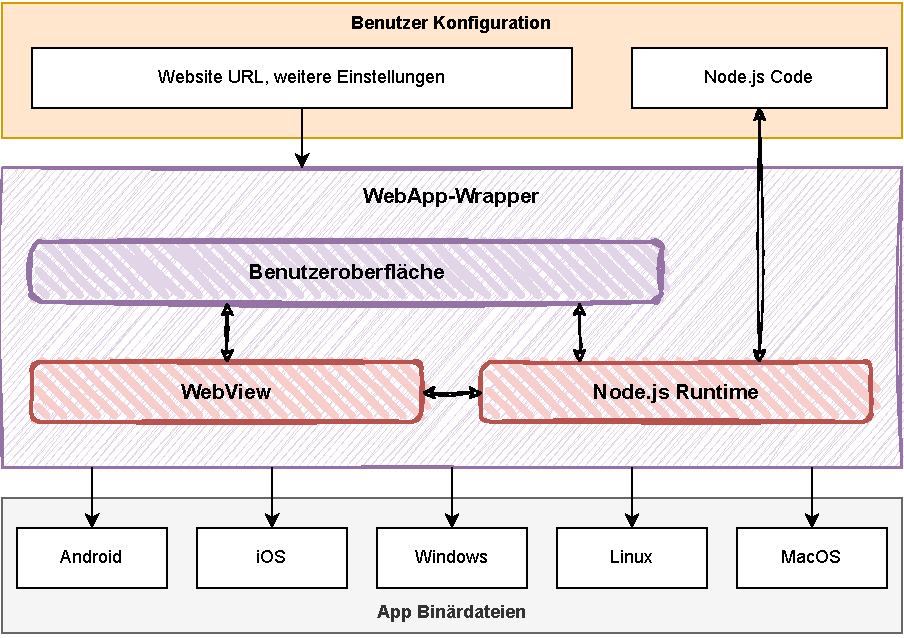
\includegraphics[width=\textwidth]{assets/04_WebApp-Wrapper/01_Zielsetzung.drawio.pdf}
\end{figure}


\clearpage

\include{src/04_WebApp-Wrapper/02_Benutzeroberfläche.tex}
\subsection{Implementation}

\begin{figure}[H]
    \centering
    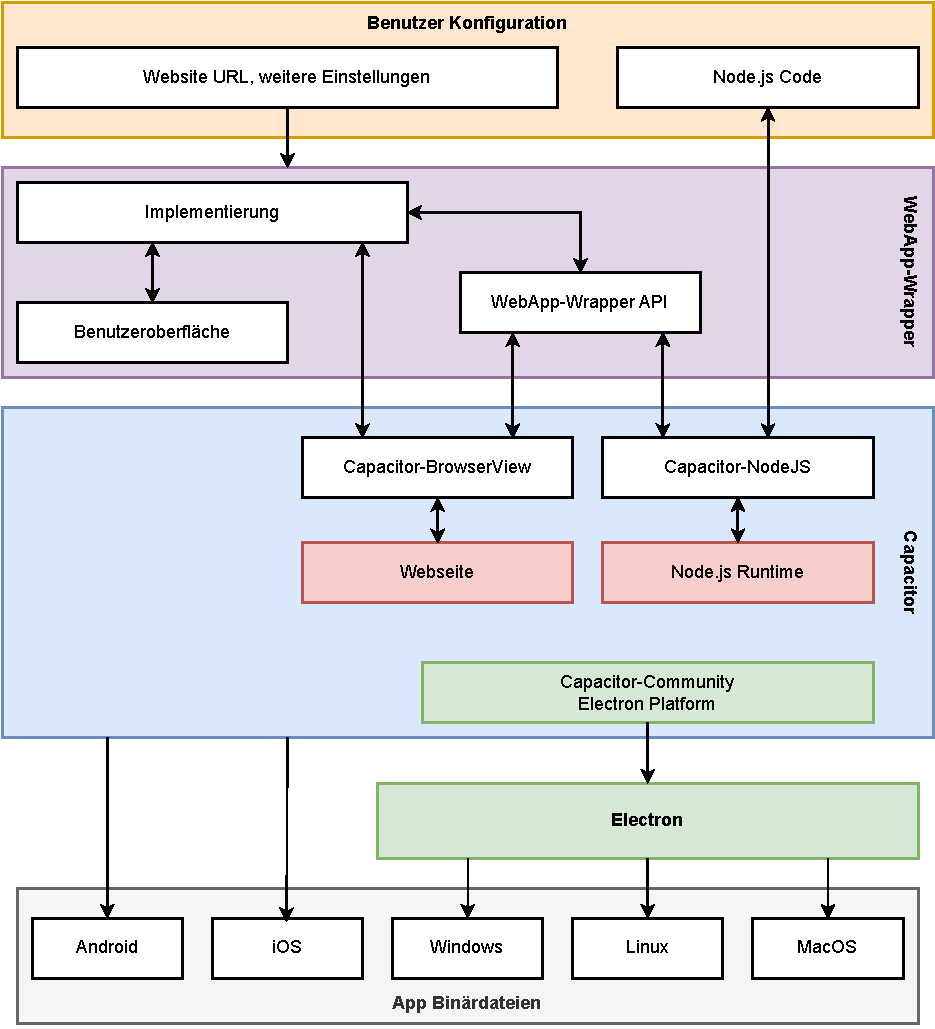
\includegraphics[width=\textwidth]{assets/04_WebApp-Wrapper/03_Aufbau.drawio.pdf}
\end{figure}


\clearpage

\subsection{Benutzung}
\label{sec:WebApp-Wrapper:Benutzung}

In diesem Kapitel wird erklärt, wie eine Anwendung mithilfe des WebApp-Wrappers erstellt werden kann.

Die neueste Version sowie die dazugehörige Dokumentation sind auf der GitHub"=Projektseite\footnote{\url{https://github.com/hampoelz/WebApp-Wrapper}} zu finden.

Da der WebApp-Wrapper auf dem Capacitor"=Framework basiert, ist es hilfreich, die Grundlagen von Capacitor zu kennen.

\subsubsection{Erste Schritte}

\paragraph{Projektdateien herunterladen}

Um mit der Erstellung einer neuen Anwendung mithilfe des WebApp-Wrappers zu beginnen, müssen zunächst die Projektdateien heruntergeladen und die Abhängigkeiten installiert werden.

Dieser Schritt ist mit den folgenden Befehlen einfach zu bewerkstelligen:

\begin{minted}[breaklines,breakafter=/]{bash}
# Lädt alle erforderlichen Dateien in den Ordner "AppProjectDir" herunter
git clone https://github.com/hampoelz/WebApp-Wrapper.git AppProjectDir

# Wechselt das Arbeitsverzeichnis in den Ordner "AppProjectDir"
cd AppProjectDir

# Installiert alle Abhängigkeiten des WebApp-Wrappers
npm install
\end{minted}

\paragraph{Konfigurationen anpassen}

Bevor die neue Anwendung gestartet werden kann, müssen zunächst die erforderlichen Konfigurationen in der Datei \code{capacitor.config.json} angepasst werden. Die folgenden Konfigurationen sind erforderlich:

\begin{itemize}
  \setlength\itemsep{-0.5em}
  \item \textbf{\code{appId}}: Eine eindeutige Anwendungs-ID
  \item \textbf{\code{appName}}: Der Name der Anwendung
  \item \textbf{\code{appUrl}}: Die \ac{url} der Webseite, die in der Anwendung angezeigt wird.
\end{itemize}

Weitere Konfigurationen können im Kapitel \nameref{sec:WebApp-Wrapper:Konfiguration} gefunden werden.

\newpage

\paragraph{Plattformen hinzufügen}

Nachdem die Konfiguration abgeschlossen ist, können Plattformen hinzugefügt werden, auf denen die Anwendung ausgeführt werden soll.

Die folgenden Befehle können verwendet werden, um Plattformen hinzuzufügen:

\begin{minted}{bash}
# Erzeugt die Projektdateien für die Plattformen
npm run build

# Fügt der Anwendung Unterstützung für eine Plattform hinzu
npx cap add <Plattform>

# Synchronisiert die Plattform mit den Projektdateien
npx cap sync <Plattform>
\end{minted}

Die verfügbaren Plattformen sind \code{android}, \code{ios} und \code{electron}.
Die Plattform \enquote{Electron} bezieht sich auf Desktop"=Plattformen, also Windows, Linux und macOS.

Wenn die Konfiguration später geändert wird, müssen die folgenden Befehle erneut ausgeführt werden:

\begin{minted}{bash}
# Aktualisiert die Projektdateien mit den neuen Konfigurationen
npm run build

# Synchronisiert die angegebenen Plattform mit den Projektdateien
npx cap sync <Plattform>
\end{minted}

\paragraph{Node.js Projekt hinzufügen}

Um zusätzliche Funktionen in die Anwendung zu integrieren, kann ein Node.js Projekt in das Verzeichnis \code{nodejs} hinzugefügt werden.
Dieses Verzeichnis ist bereits vorkonfiguriert, sodass ein Node.js Projekt einfach integrieren werden kann.

Nach dem Hinzufügen oder Ändern des Node.js Projekts müssen die folgenden Befehle ausgeführt werden, um die Projektdateien zu aktualisieren:

\begin{minted}{bash}
# Aktualisiert die Projektdateien mit dem Node.js Projekt
npm run build

# Synchronisiert die Plattform mit den Projektdateien
npx cap sync <Plattform>
\end{minted}

\newpage

\paragraph{Anwendung starten}

Um die Anwendung schließlich zu starten, kann der folgende Befehl verwendet werden.

\begin{minted}{bash}
# Öffnet das Projekt für die angegebene Plattform
npx cap open <Plattform>
\end{minted}

Dieser Befehl öffnet das Projekt für die angegebene Plattform in der entsprechenden Entwicklungsumgebung. 
Bei Android und iOS wird Android Studio bzw.\ Xcode geöffnet, wenn diese auf dem System installiert sind.
In der Entwicklungsumgebung können weitere Aktionen durchgeführt werden, wie das Testen im Emulator, das Debuggen oder das Kompilieren.

Alternativ kann das Projekt für eine Plattform auch manuell geöffnet werden. Die entsprechenden Plattform"=Projektdateien befinden sich in den Verzeichnissen \code{android} und \code{ios}.

Bei Electron wird die Anwendung direkt gestartet. Weitere Aktionen können dabei im Plattform"=Projektordner \code{electron} durchgeführt werden.


\clearpage

\subsubsection{Konfiguration}
\label{sec:WebApp-Wrapper:Konfiguration}

Die folgenden Konfigurationen sind verfügbar:

\begin{configuration}{WebApp-Wrapper / Konfiguration}
  \code{appId}        & \code[typescript]{string}     & Ein eindeutiger Bezeichner für die Anwendung. Sie wird auch als Bundle-ID in iOS und als Anwendungs-ID in Android bezeichnet. Sie muss in umgekehrter Domänennamenschreibweise angegeben werden, was im Allgemeinen einen Domänennamen darstellt, der dem Unternehmen gehört.\\ \hline
  \code{appName}      & \code[typescript]{string}     & Der benutzerfreundliche Name der Anwendung. Dies sollte der Name sein, der im AppStore angezeigt wird. \\ \hline
  \code{appUrl}       & \code[typescript]{string}     & Die Adresse der Webseite, die in der Anwendung angezeigt wird. \\ \hline
  \code{primaryColor} & \code[typescript]{string}     & Die Hauptfarbe der Benutzeroberfläche. Der Standardwert ist \textcolor[HTML]{BB4747}{\code*{"\#1095c1"}} \\ \hline
  \code{menuColor}    & \code[typescript]{string}     & Die Hintergrundfarbe der Menüleiste. \\ \hline
  \code{menu}         & \code[typescript]{MenuItem[]} & Eine Liste von Menüelementen. Jedes angegebene Menüelement wird in der Menüleiste angezeigt. Wenn diese Konfiguration nicht festgelegt wurde, wird keine Menüleiste angezeigt. \\ \hline
  \code{contactUrl}   & \code[typescript]{string}     & Eine Webseite, unter der ein Fehlerbericht erstellt werden kann, wenn die angegebene Webseite aufgrund eines Serverfehlers nicht geladen werden kann. \\ \hline
\end{configuration}

\newpage

\textbf{Beispiele}

In \code{capacitor.config.json}:

\begin{minted}{json}
{
  "appId": "com.company.app",
  "appName": "Company App",
  "appUrl": "https://app.company.com/",
  "primaryColor": "#1b66c9",
  "menuColor": "#202124",
  "menu": [
    {
      "id": "test-button",
      "type": "button",
      "text": "Hello World"
    }
  ],
  "contactUrl": "",
  "webDir": "dist"
}
\end{minted}

\begin{warning}
    Die Konfiguration \code{webDir} darf nicht verändert werden.
    Capacitor verwendet diese Konfiguration, um die Plattformen mit den Projektdateien zu synchronisieren.
    Wenn Sie diese Konfiguration ändern, kann es zu Problemen bei der Synchronisierung kommen.
\end{warning}

\clearpage

\subsubsection{API - Node.js Projekt}

Der WebApp-Wrapper bietet im Node.js Projekt eine \ac{api} an, um Konfigurationen zu ändern, die Webseite zu steuern und Nachrichten zwischen dem Node.js Projekt und der Webseite auszutauschen.

Die \acs{api}-Methoden sind über das Modul \code{bridge} verfügbar.
Es verfügt über die folgenden Methoden:

\begin{itemize}
  \setlength\itemsep{-0.8em}
  \item \code{channel.send('wrapper:updateColor', ...)}
  \item \code{channel.send('wrapper:updateMenuColor', ...)}
  \item \code{channel.send('wrapper:enableMenu', ...)}
  \item \code{channel.send('wrapper:addMenuItem', ...)}
  \item \code{channel.send('wrapper:removeMenuItem', ...)}
  \item \code{channel.send('wrapper:openMessageScreen', ...)}
  \item \code{channel.send('wrapper:closeMessageScreen')}
  \item \code{channel.send('wrapper:sendMessage', ...)}
  \item \code{channel.addListener('wrapper:onMessage', ...)}
  \item \code{channel.addListener('wrapper:onMenuClick', ...)}
\end{itemize}

\begin{itemize}
  \setlength\itemsep{-0.8em}
  \item \code{channel.send('wrapper:loadUrl', ...)}
  \item \code{channel.send('wrapper:reload')}
  \item \code{channel.send('wrapper:clearHistory')}
  \item \code{channel.send('wrapper:goBack')}
  \item \code{channel.send('wrapper:goForward')}
  \item \code{channel.send('wrapper:executeJavaScript', ...)}
  \item \code{channel.addListener('will-navigate', ...)}
  \item \code{channel.addListener('did-start-loading', ...)}
  \item \code{channel.addListener('did-finish-load', ...)}
  \item \code{channel.addListener('did-fail-load', ...)}
  \item \code{channel.addListener('dom-ready', ...)}
\end{itemize}

\begin{itemize}
  \setlength\itemsep{-0.8em}
  \item Interfaces
\end{itemize}

% -------------------- %

\paragraph{channel.send('wrapper:updateColor', ...)}

\begin{minted}{typescript}
  send: (
    eventName: 'wrapper:updateColor',
    color: string
  ) => void
\end{minted}

Aktualisiert die Hauptfarbe der Benutzeroberfläche.

\begin{arguments}
  \item \code{color}: Die neue Hauptfarbe im \code*{\#RRGGBB}-Format.
\end{arguments}

% -------------------- %

\newpage

\paragraph{channel.send('wrapper:updateMenuColor', ...)}

\begin{minted}{typescript}
  send: (
    eventName: 'wrapper:updateMenuColor',
    color: string
  ) => void
\end{minted}

Ändert die Hintergrundfarbe der Menüleiste.

\begin{arguments}
  \item \code{color}: Die neue Hintergrundfarbe im \code*{\#RRGGBB}-Format.
\end{arguments}

% -------------------- %

\paragraph{channel.send('wrapper:enableMenu', ...)}

\begin{minted}{typescript}
  send: (
    eventName: 'wrapper:enableMenu',
    enable: boolean
  ) => void
\end{minted}

Aktiviert oder deaktiviert die Menüleiste.

\begin{arguments}
  \item \code{enable}: \code[javascript]{true}, um die Menüleiste zu aktivieren. \code[javascript]{false}, um sie zu deaktivieren.
\end{arguments}

% -------------------- %

\paragraph{channel.send('wrapper:addMenuItem', ...)}

\begin{minted}{typescript}
  send: (
    eventName: 'wrapper:addMenuItem',
    item: MenuItem
  ) => void
\end{minted}

Fügt ein \code*{MenuItem} zur Menüleiste hinzu.

\begin{arguments}
  \item \code{item}: Das Menüelement, das hinzugefügt werden soll.
\end{arguments}

% -------------------- %

\paragraph{channel.send('wrapper:removeMenuItem', ...)}

\begin{minted}{typescript}
  send: (
    eventName: 'wrapper:removeMenuItem',
    itemId: string
  ) => void
\end{minted}

Entfernt ein Menüelement mit der eindeutigen ID \code{itemId} aus der Menüleiste.

\begin{arguments}
  \item \code{itemId}: Die ID des Menüelements, das entfernt werden soll.
\end{arguments}

% -------------------- %

\newpage

\paragraph{channel.send('wrapper:openMessageScreen', ...)}

\begin{minted}{typescript}
  send: (
    eventName: 'wrapper:openMessageScreen',
    html: string
  ) => void
\end{minted}

Öffnet oder aktualisiert das Meldungsfenster.
Es kann mit \ac{html} angepasst werden und wird automatisch mit Stilen des PicoCSS Frameworks versehen.

\begin{arguments}
  \item \code{html}: Der \ac{html}-Code für das Meldungsfenster.
\end{arguments}

% -------------------- %

\paragraph{channel.send('wrapper:closeMessageScreen')}

\begin{minted}{typescript}
  send: (
    eventName: 'wrapper:closeMessageScreen'
  ) => void
\end{minted}

Schließt das Meldungsfenster.

% -------------------- %

\paragraph{channel.send('wrapper:sendMessage', ...)}

\begin{minted}{typescript}
  send: (
    eventName: 'wrapper:updateColor',
    ...args: any[]
  ) => void
\end{minted}

Sendet eine Nachricht an die Webseite zusammen mit Argumenten.
Die Argumente werden mit \ac{json} serialisiert.

\begin{arguments}
  \item \code{args}: Eine Liste der Argumente, die gesendet werden sollen.
\end{arguments}

% -------------------- %

\paragraph{channel.addListener('wrapper:onMessage', ...)}

\begin{minted}{typescript}
  addListener: (
    eventName: 'wrapper:onMessage',
    listener: (...args: any[]) => void
  ) => void
\end{minted}

Ruft \code{listener(args...)} auf, wenn eine neue Nachricht von der Webseite eintrifft.

\begin{arguments}
  \item \code{args}: Eine Liste der Argumente, die empfangenen wurden.
\end{arguments}

% -------------------- %

\newpage

\paragraph{channel.addListener('wrapper:onMenuClick', ...)}

\begin{minted}{typescript}
  addListener: (
    eventName: 'wrapper:onMenuClick',
    listener: (itemId: string) => void
  ) => void
\end{minted}

Ruft \code{listener(data)} auf, wenn auf eine Schaltfläche in der Menüleiste geklickt wurde.

\begin{arguments}
  \item \code{itemId}: Die ID des Menüelements, das angeklickt wurde.
\end{arguments}

% -------------------- %


%! The following APIs are forwarded from the Capacitor-BrowserView plugin
% -------------------- %

\paragraph{channel.send('wrapper:loadUrl', ...)}

\begin{minted}{typescript}
  send(
    eventName: 'wrapper:loadUrl',
    url: string
  ) => void
\end{minted}

Lädt die angegebene \ac{url} in die Ansicht.
Die \ac{url} muss einen Protokollpräfix enthalten, z.B.\ den \code{https://}.

\begin{arguments}
  \item \code{url}: Die \ac{url} einer Webseite.
\end{arguments}

% -------------------- %

\paragraph{channel.send('wrapper:reload')}

\begin{minted}{typescript}
  send(
    eventName: 'wrapper:reload'
  ) => void
\end{minted}

Lädt die aktuelle Webseite neu.

% -------------------- %

\paragraph{channel.send('wrapper:clearHistory')}

\begin{minted}{typescript}
  send(
    eventName: 'wrapper:clearHistory'
  ) => void
\end{minted}

Löscht die interne Liste der Rück- und Vorwärtsnavigation.

% -------------------- %

\paragraph{channel.send('wrapper:goBack')}

\begin{minted}{typescript}
  send(
    eventName: 'wrapper:goBack'
  ) => void
\end{minted}

Bringt den Browser dazu, eine Webseite zurückzugehen.

% -------------------- %

\newpage

\paragraph{channel.send('wrapper:goForward')}

\begin{minted}{typescript}
  send(
    eventName: 'wrapper:goForward'
  ) => void
\end{minted}

Bringt den Browser dazu, eine Webseite weiterzuleiten.

% -------------------- %

\paragraph{channel.send('wrapper:executeJavaScript', ...)}

\begin{minted}{typescript}
  send(
    eventName: 'wrapper:executeJavaScript',
    code: string
  ) => void
\end{minted}

Führt JavaScript asynchron im Kontext der aktuell angezeigten Webseite aus.

\begin{arguments}
  \item \code{code}: Der JavaScript-Code, der ausgeführt werden soll.
\end{arguments}

% -------------------- %

\paragraph{channel.addListener('will-navigate', ...)}

\begin{minted}{typescript}
  addListener(
    eventName: 'will-navigate',
    listenerFunc: (
      url: string,
      isExternal: boolean
    ) => void
  ) => void
\end{minted}

Ruft \code{listenerFunc(data)} auf, wenn ein Benutzer oder die Webseite eine Navigation starten will.
Dies kann geschehen, wenn das Objekt \code[javascript]{window.location} geändert wird oder ein Benutzer auf einen Link auf der Webseite klickt.

Dieses Ereignis wird nicht ausgelöst, wenn die Navigation programmgesteuert mit \acsp{api} gestartet wird, wie \code{wrapper:loadUrl} und \code{wrapper:goBack}, oder für POST"=Anfragen.

Es wird auch nicht für seiteninterne Navigationen ausgelöst, wie das Anklicken von Ankerlinks oder die Aktualisierung des \code[javascript]{window.location.hash}.

\begin{arguments}
  \item \code{url}: Die \ac{url} einer Webseite.
  \item \code{isExternal}: Ob die \ac{url} im externen Browser oder in der BrowserView geöffnet wird.
\end{arguments}

% -------------------- %

\newpage

\paragraph{channel.addListener('did-start-loading', ...)}

\begin{minted}{typescript}
  addListener(
    eventName: 'did-start-loading',
    listenerFunc: () => void
  ) => void
\end{minted}

Ruft \code{listenerFunc()} auf, wenn die Webseite mit dem Laden begonnen hat.

% -------------------- %

\paragraph{channel.addListener('did-finish-load', ...)}

\begin{minted}{typescript}
  addListener(
    eventName: 'did-finish-load',
    listenerFunc: () => void
  ) => void
\end{minted}

Ruft \code{listenerFunc()} auf, wenn das Laden der Webseite abgeschlossen ist.
Dies garantiert nicht, dass der nächste gezeichnete Frame den Zustand des \ac{dom} zu diesem Zeitpunkt wiedergibt.

% -------------------- %

\paragraph{channel.addListener('did-fail-load', ...)}

\begin{minted}{typescript}
  addListener(
    eventName: 'did-fail-load',
    listenerFunc: (error: WebResourceError) => void
  ) => void
\end{minted}

Ruft \code{listenerFunc(data)} auf, wenn die Webseite nicht geladen werden kann.
Diese Fehler weisen in der Regel darauf hin, dass keine Verbindung zum Server hergestellt werden kann.

\begin{arguments}
  \item \code{error}: Informationen über den aufgetretenen Fehler.
\end{arguments}

% -------------------- %

\paragraph{channel.addListener('dom-ready', ...)}

\begin{minted}{typescript}
  addListener(
    eventName: 'dom-ready',
    listenerFunc: () => void
  ) => void
\end{minted}

Ruft \code{listenerFunc()} auf, wenn das Dokument im Frame der obersten Ebene geladen wurde.

% -------------------- %

\newpage

\paragraph{Interfaces}

% -------------------- %

\subparagraph{MenuItem}

Ein Interface, das Informationen über einen Menüelement enthält.

\begin{interfacedesc}{WebApp-Wrapper / MenuItem (Node.js Projekt API)}
  \code{id}   & \code[typescript]{string} & Eine eindeutige ID für das Menüelement. \\ \hline
  \code{type} & \code[typescript]{string} & Der Anzeigetyp des Menüelements. Die folgenden Typen sind verfügbar: \\
              &                           & \textbf{\code{text}}: Ein einfaches Textelement. \\
              &                           & \textbf{\code{separator}}: Ein Trennstrich. \\
              &                           & \textbf{\code{button}}: Eine Schaltfläche mit Text. \\
              &                           & \textbf{\code{button_primary}}: Eine Schaltfläche mit Text und hervorgehobener Farbe. \\ \hline
  \code{text} & \code[typescript]{string} & Der Text, der in der Menüleiste für dieses Element angezeigt wird. \\ \hline
\end{interfacedesc}

\subparagraph{WebResourceError}

Ein Interface, das Informationen über den Fehler enthält, der beim Laden von Webressourcen aufgetreten ist.

\begin{interfacedesc}{WebApp-Wrapper / WebResourceError}
  errorCode         & \code[typescript]{string} & Der Fehlercode des Fehlers. \\ \hline
  errorDescription  & \code[typescript]{string} & Eine Zeichenfolge, die den Fehler beschreibt. Beschreibungen sind lokalisiert und können daher verwendet werden, um dem Benutzer das Problem mitzuteilen. \\ \hline
  validatedURL      & \code[typescript]{string} & Die \ac{url}, die nicht geladen werden konnte. \\ \hline
\end{interfacedesc}

\clearpage

\subsubsection{API - Webseite}

Der WebApp-Wrapper bietet auf der Webseite eine \ac{api} an, um Konfigurationen zu ändern und Nachrichten zwischen der Webseite und dem Node.js Projekt auszutauschen.

Die folgenden Methoden stehen zur Verfügung:

\begin{itemize}
  \setlength\itemsep{-0.8em}
  \item \code{CapacitorBrowserView.send('wrapper:updateColor', ...)}
  \item \code{CapacitorBrowserView.send('wrapper:updateMenuColor', ...)}
  \item \code{CapacitorBrowserView.send('wrapper:enableMenu', ...)}
  \item \code{CapacitorBrowserView.send('wrapper:addMenuItem', ...)}
  \item \code{CapacitorBrowserView.send('wrapper:removeMenuItem', ...)}
  \item \code{CapacitorBrowserView.send('wrapper:openMessageScreen', ...)}
  \item \code{CapacitorBrowserView.send('wrapper:closeMessageScreen')}
  \item \code{CapacitorBrowserView.send('wrapper:sendMessage', ...)}
  \item \code{CapacitorBrowserView.addListener('wrapper:onMessage', ...)}
  \item \code{CapacitorBrowserView.addListener('wrapper:onMenuClick', ...)}
  \item Interfaces
\end{itemize}

% -------------------- %

\paragraph{CapacitorBrowserView.send('wrapper:updateColor', ...)}

\begin{minted}{typescript}
  send: (
    eventName: 'wrapper:updateColor',
    color: string
  ) => void
\end{minted}

Aktualisiert die Hauptfarbe der Benutzeroberfläche.

\begin{arguments}
  \item \code{color}: Die neue Hauptfarbe im \code*{\#RRGGBB}-Format.
\end{arguments}

% -------------------- %

\paragraph{CapacitorBrowserView.send('wrapper:updateMenuColor', ...)}

\begin{minted}{typescript}
  send: (
    eventName: 'wrapper:updateMenuColor',
    color: string
  ) => void
\end{minted}

Ändert die Hintergrundfarbe der Menüleiste.

\begin{arguments}
  \item \code{color}: Die neue Hintergrundfarbe im \code*{\#RRGGBB}-Format.
\end{arguments}

% -------------------- %

\newpage

\paragraph{CapacitorBrowserView.send('wrapper:enableMenu', ...)}

\begin{minted}{typescript}
  send: (
    eventName: 'wrapper:enableMenu',
    enable: boolean
  ) => void
\end{minted}

Aktiviert oder deaktiviert die Menüleiste.

\begin{arguments}
  \item \code{enable}: \code[javascript]{true}, um die Menüleiste zu aktivieren. \code[javascript]{false}, um sie zu deaktivieren.
\end{arguments}

% -------------------- %

\paragraph{CapacitorBrowserView.send('wrapper:addMenuItem', ...)}

\begin{minted}{typescript}
  send: (
    eventName: 'wrapper:addMenuItem',
    item: MenuItem
  ) => void
\end{minted}

Fügt ein Menüelement zur Menüleiste hinzu.

\begin{arguments}
  \item \code{item}: Das Menüelement \code*{MenuItem}, das hinzugefügt werden soll.
\end{arguments}

% -------------------- %

\paragraph{CapacitorBrowserView.send('wrapper:removeMenuItem', ...)}

\begin{minted}{typescript}
  send: (
    eventName: 'wrapper:removeMenuItem',
    itemId: string
  ) => void
\end{minted}

Entfernt ein Menüelement mit der eindeutigen ID \code{itemId} aus der Menüleiste.

\begin{arguments}
  \item \code{itemId}: Die ID des Menüelements, das entfernt werden soll.
\end{arguments}

% -------------------- %

\paragraph{CapacitorBrowserView.send('wrapper:openMessageScreen', ...)}

\begin{minted}{typescript}
  send: (
    eventName: 'wrapper:openMessageScreen',
    html: string
  ) => void
\end{minted}

Öffnet oder aktualisiert das Meldungsfenster.
Es kann mit \ac{html} angepasst werden und wird automatisch mit Styles des PicoCSS Frameworks versehen.

\begin{arguments}
  \item \code{html}: Der \ac{html}-Code für das Meldungsfenster.
\end{arguments}

% -------------------- %

\newpage

\paragraph{CapacitorBrowserView.send('wrapper:closeMessageScreen')}

\begin{minted}{typescript}
  send: (
    eventName: 'wrapper:closeMessageScreen'
  ) => void
\end{minted}

Schließt das Meldungsfenster.

% -------------------- %

\paragraph{CapacitorBrowserView.send('wrapper:sendMessage', ...)}

\begin{minted}{typescript}
  send: (
    eventName: 'wrapper:updateColor',
    ...args: any[]
  ) => void
\end{minted}

Sendet eine Nachricht an das Node.js Projekt zusammen mit Argumenten.
Die Argumente werden mit \ac{json} serialisiert.

\begin{arguments}
  \item \code{args}: Eine Liste der Argumente, die gesendet werden sollen.
\end{arguments}

% -------------------- %

\paragraph{CapacitorBrowserView.addListener('wrapper:onMessage', ...)}

\begin{minted}{typescript}
  addListener: (
    eventName: 'wrapper:onMessage',
    listener: (...args: any[]) => void
  ) => void
\end{minted}

Ruft \code{listener(args...)} auf, wenn eine neue Nachricht von dem Node.js Projekt eintrifft.

\begin{arguments}
  \item \code{args}: Eine Liste der Argumente, die empfangenen wurden.
\end{arguments}

% -------------------- %

\paragraph{CapacitorBrowserView.addListener('wrapper:onMenuClick', ...)}

\begin{minted}{typescript}
  addListener: (
    eventName: 'wrapper:onMenuClick',
    listener: (itemId: string) => void
  ) => void
\end{minted}

Ruft \code{listener(data)} auf, wenn auf eine Schaltfläche in der Menüleiste geklickt wurde.

\begin{arguments}
  \item \code{itemId}: Die ID des Menüelements, das angeklickt wurde.
\end{arguments}

% -------------------- %

\newpage

\paragraph{Interfaces}

% -------------------- %

\subparagraph{MenuItem}

Ein Interface, das Informationen über ein Menüelement enthält.

\begin{interfacedesc}{WebApp-Wrapper / MenuItem (Webseite API)}
  \code{id}   & \code[typescript]{string} & Eine eindeutige ID für das Menüelement. \\ \hline
  \code{type} & \code[typescript]{string} & Der Anzeigetyp des Menüelements. Die folgenden Typen sind verfügbar: \\
              &                           & \textbf{\code{text}}: Ein einfaches Textelement. \\
              &                           & \textbf{\code{separator}}: Ein Trennstrich. \\
              &                           & \textbf{\code{button}}: Eine Schaltfläche mit Text. \\
              &                           & \textbf{\code{button_primary}}: Eine Schaltfläche mit Text und hervorgehobener Farbe. \\ \hline
  \code{text} & \code[typescript]{string} & Der Text, der in der Menüleiste für dieses Element angezeigt wird. \\ \hline
\end{interfacedesc}

\clearpage

\subsubsection{API - Meldungsfenster}

Der WebApp-Wrapper bietet im Meldungsfenster eine \ac{api} an, das Meldungsfenster wieder zu schließen und Nachrichten an das Node.js Projekt oder an die Webseite zu senden.

Die folgenden Methoden stehen zur Verfügung:

\begin{itemize}
  \setlength\itemsep{-0.8em}
  \item \code{closeMessageScreen()}
  \item \code{sendMessage(...)}
\end{itemize}

% -------------------- %

\paragraph{closeMessageScreen()}

\begin{minted}{typescript}
  closeMessageScreen: () => void
\end{minted}

Schließt das Meldungsfenster.

% -------------------- %

\paragraph{sendMessage(...)}

\begin{minted}{typescript}
  sendMessage: (
    receiver: 'nodejs' | 'pwa',
    ...args: any[]
  ) => void
\end{minted}

Sendet eine Nachricht an das Node.js Projekt oder and die Webseite zusammen mit Argumenten.
Die Argumente werden mit \ac{json} serialisiert.

\begin{itemize}
  \setlength\itemsep{-0.5em}
  \item \code{receiver}: Der Empfänger der Nachricht.\\
    \hspace*{1em} Die folgenden Werte werden akzeptiert:\\
    \hspace*{1em}\code{nodejs}: Sendet die Nachricht an das Node.js Projekt\\
    \hspace*{1em}\code{pwa}: Sendet die Nachricht an die Webseite
  \item \code{args}: Eine Liste der Argumente, die gesendet werden sollen.
\end{itemize}




\printLiteratur     % Literatur
\printAbbildungen   % Abbildungsverzeichnis
\printTabellen      % Tabellenverzeichnis
\printAkronyme      % Abkürzungsverzeichnis
\printAppendix      % Anhang
\printFullChangelog % Vollständiger Änderungsverlauf

\end{document}